
%%%%%%%%%%%%%%%%%%%%%%%%%%%%%%%%%%%%%%%%%%%%%%%%%%%%%%%%%%%%%%%%%%% 
%                                                                 %
%                           RESULTS                               %
%                                                                 %
%%%%%%%%%%%%%%%%%%%%%%%%%%%%%%%%%%%%%%%%%%%%%%%%%%%%%%%%%%%%%%%%%%% 
 
% \specialhead{INTRODUCTION}
\chapter{RESULTS}
\label{chapter:results}

In the previous two chapters, we discussed the changes to the overall visualization systems as well as the methods to perform non-linear magnification on our dataset. This chapter presents the resulting visualization of the entire application, various performance statistics, and a brief survey of opinions regarding the magnification effect.

\section{Images}
\label{section:image_results}

Figure~\ref{fig:s_r_no_zoom} displays the visualization of an area of just the road network and satellite images. This image is what is stored in the FBO while this region is being viewed. Figure~\ref{fig:s_r_mag} shows successively higher levels of magnification around a single cursor. The red and blue visualization is a debugging tool to indicate which areas are under linear magnification (red) and which are under non-linear magnification (blue). The outer radius is set to 400 pixels and the inner is set at 200 pixels for these images. As the magnification increases, the area being magnified becomes more pixelated. This is due to the limited resolution of the original texture stored in the FBO\@. As we perform magnification, fewer individual pixels of the source texture are being used for the same region. 

To provide a high resolution image at these high levels of magnification, we can render the scene multiple times based on the different magnification levels utilized by the users. If we attempt to store the same geographic layer at $n$ times the current level of detail, we produce an image that is $n^2$ as big as the current texture. We are using RGB values for the texture, which results in $3 * width * height$ bytes for each original texture with a viewport of $width$ by $height$ pixels. We currently run the application at a 1600 x 1000 resolution, which requires 4.5 MB of data on the GPU\@. Most modern GPUs allow for between 2 GB to 4 GB
of data on the GPU at any time; this means that we cannot simply render all the data to the GPU for a given geographic region, as we currently allow for a 72x linear magnification. This magnification would require 22 GB of storage on the GPU.

We can begin to avoid this memory issue by only storing the higher resolution images in regions that are near cursors. However, there still may be problems with performing this rendering multiple times for each cursor, for each frame. Currently, we allow for 45 discrete levels of linear magnification, so we should only calculate these high resolution region for the current level of linear magnification of the cursor  as well as its neighboring values. 

\begin{figure}[htp] \centering
    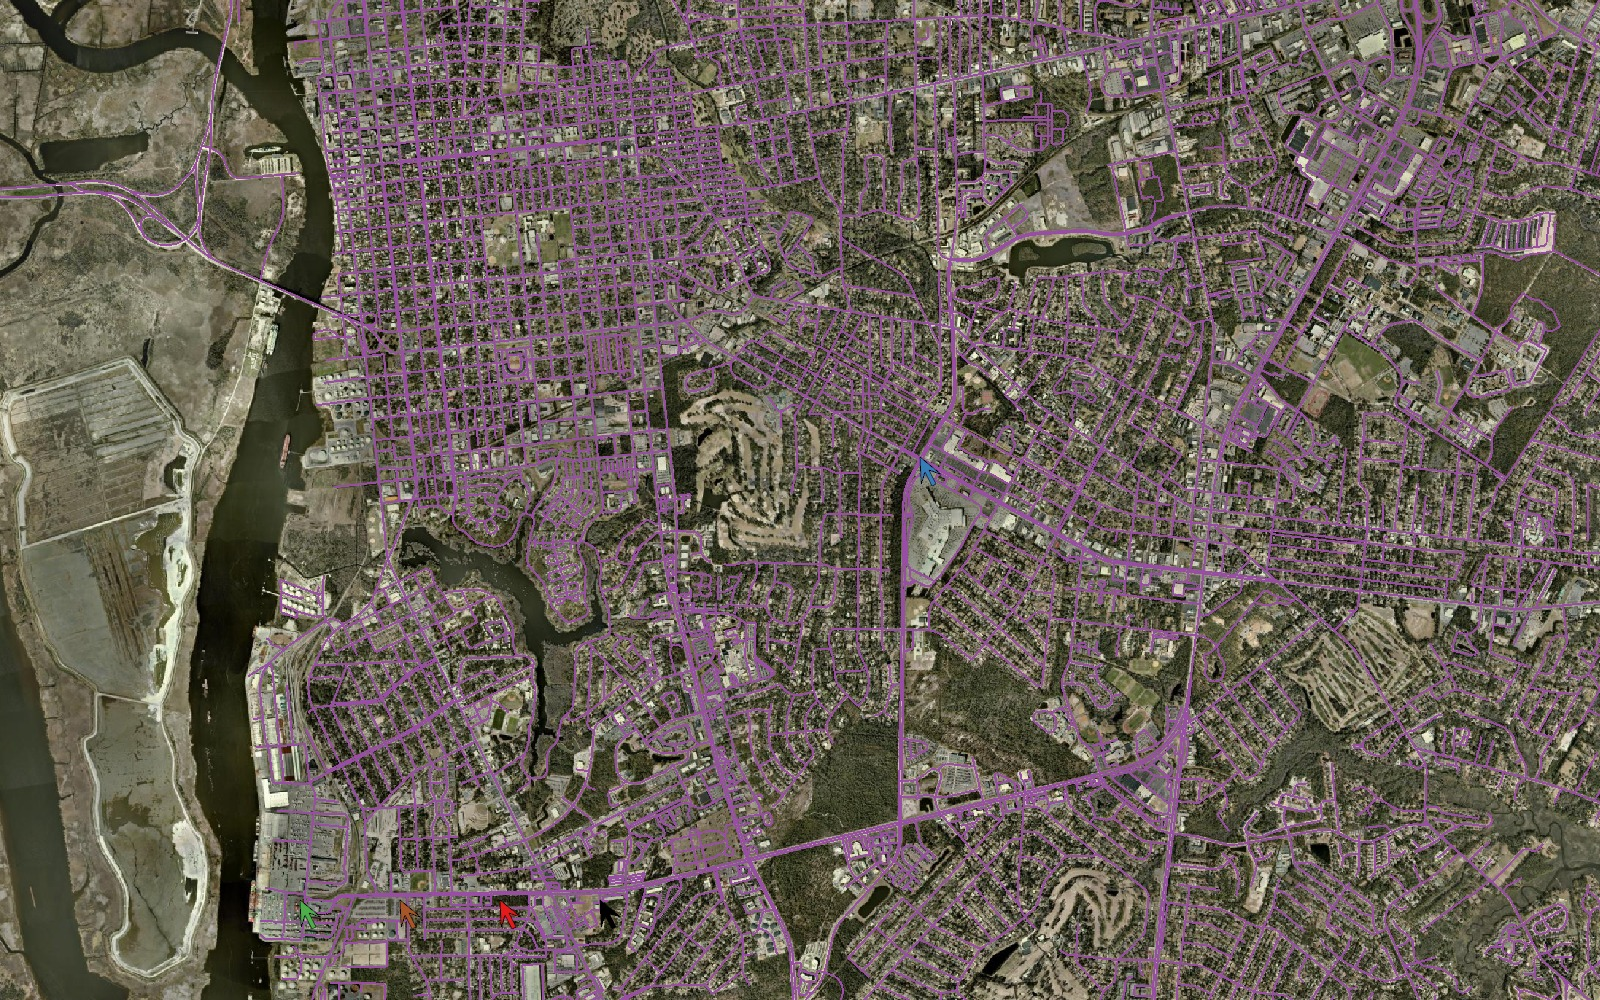
\includegraphics[width=1.0\linewidth]{img/s_r_no_zoom.jpg}
    \caption[Satellite Images and Road Network without Magnification]{A single image showing a section of the application with just the road network and satellite images. This is the current contents of the FBO, and is transformed by the magnification functions to produce the images in Figure~\ref{fig:s_r_mag}.}
    \label{fig:s_r_no_zoom}
\end{figure}

\begin{figure}[htp] \centering
    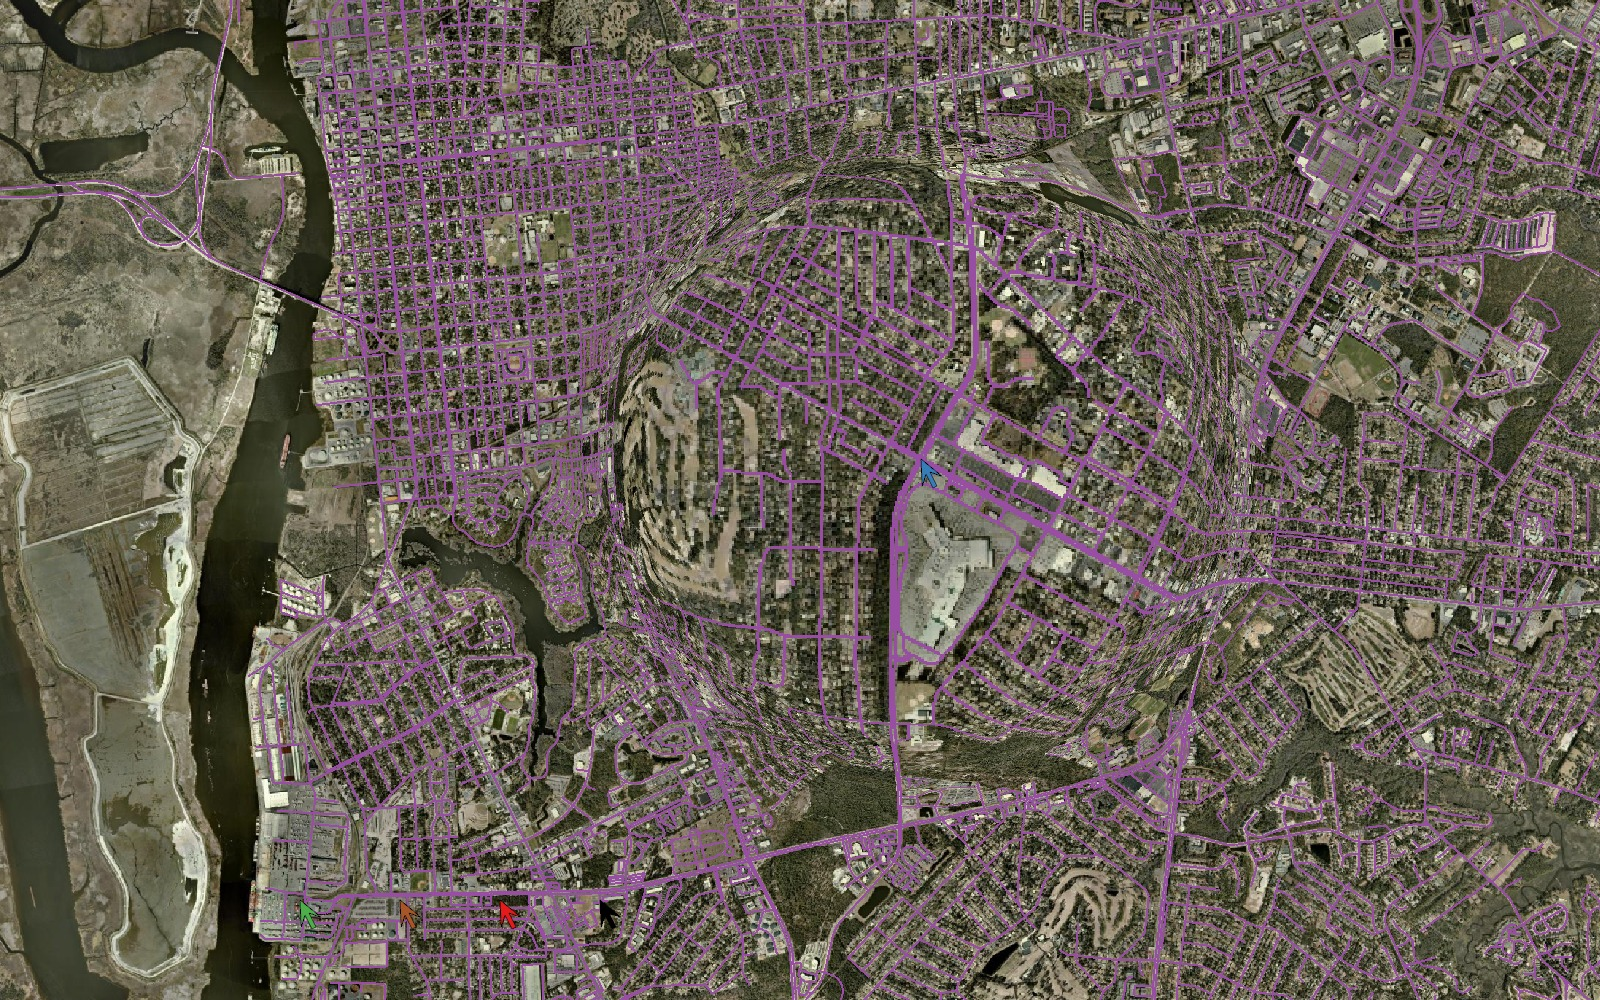
\includegraphics[width=0.49\linewidth]{img/s_r_5_zoom.jpg}
    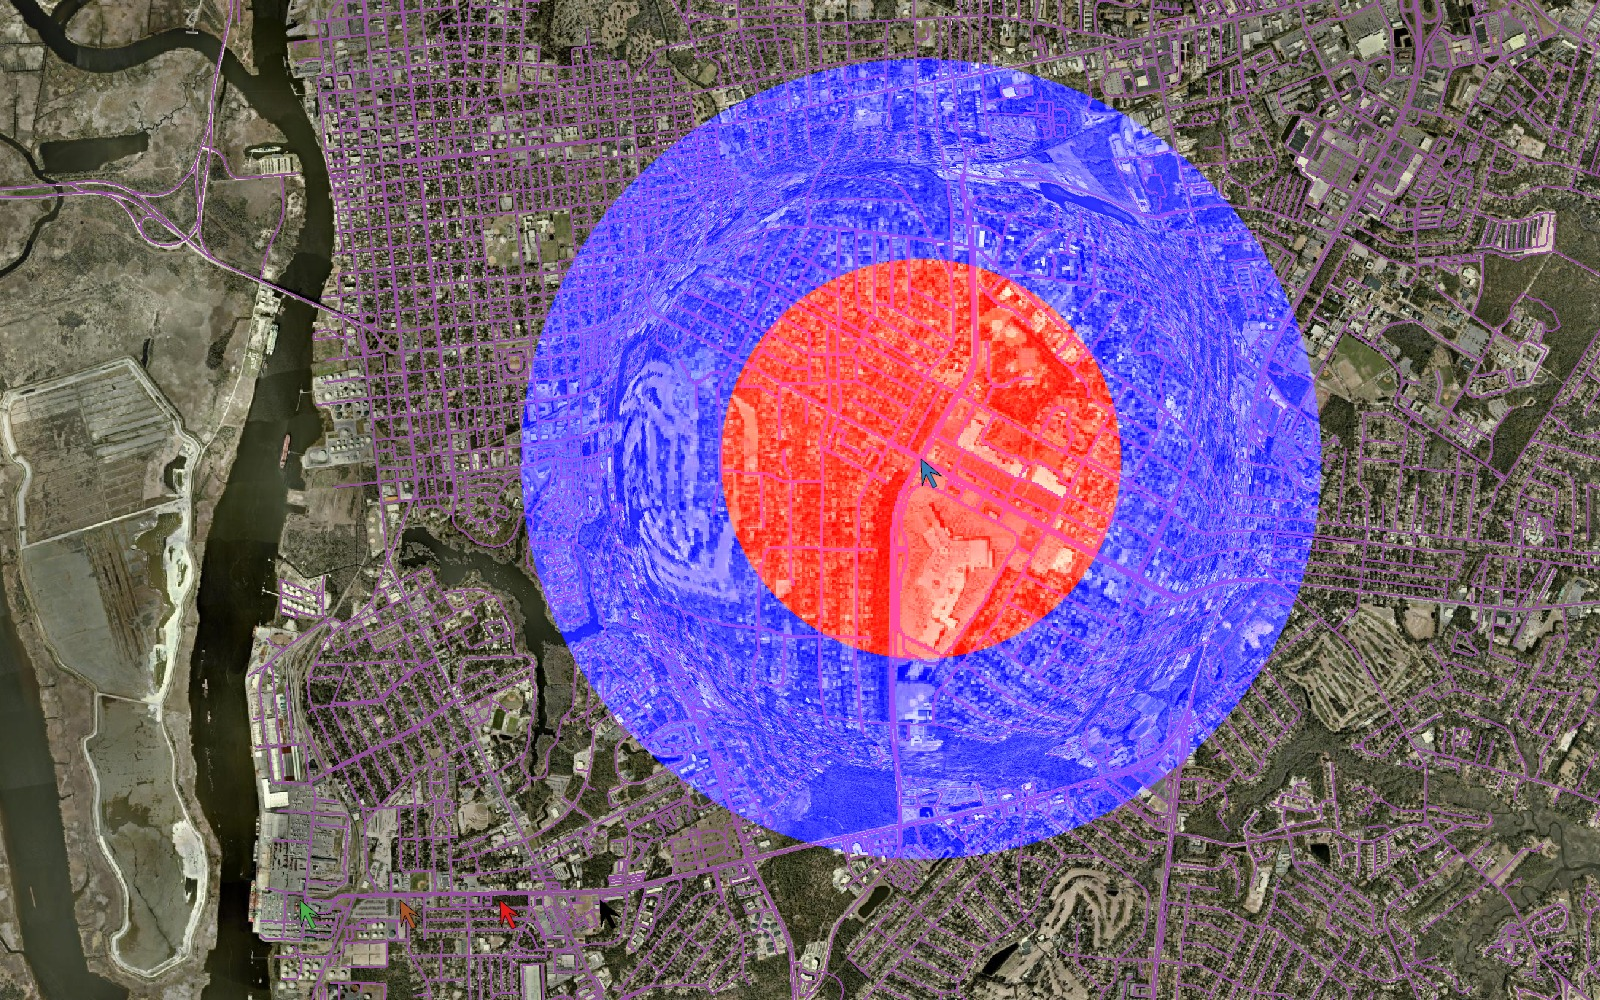
\includegraphics[width=0.49\linewidth]{img/s_r_5_zoom_color.jpg}
    \vspace{3 mm}

    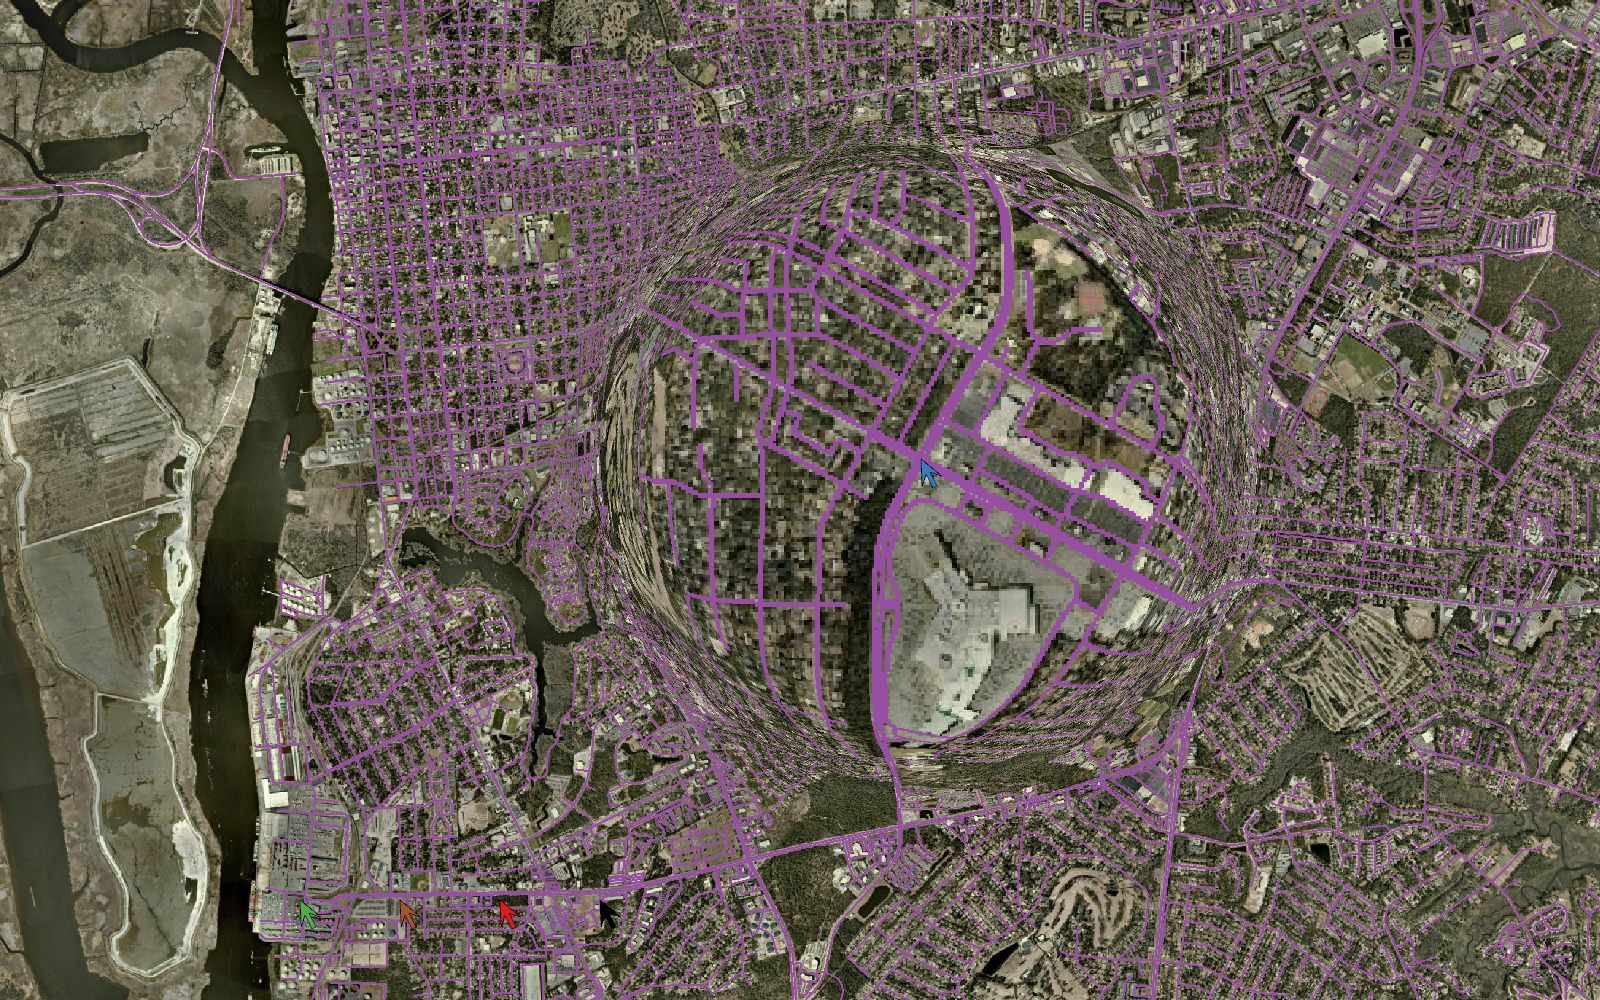
\includegraphics[width=0.49\linewidth]{img/s_r_10_zoom.jpg}
    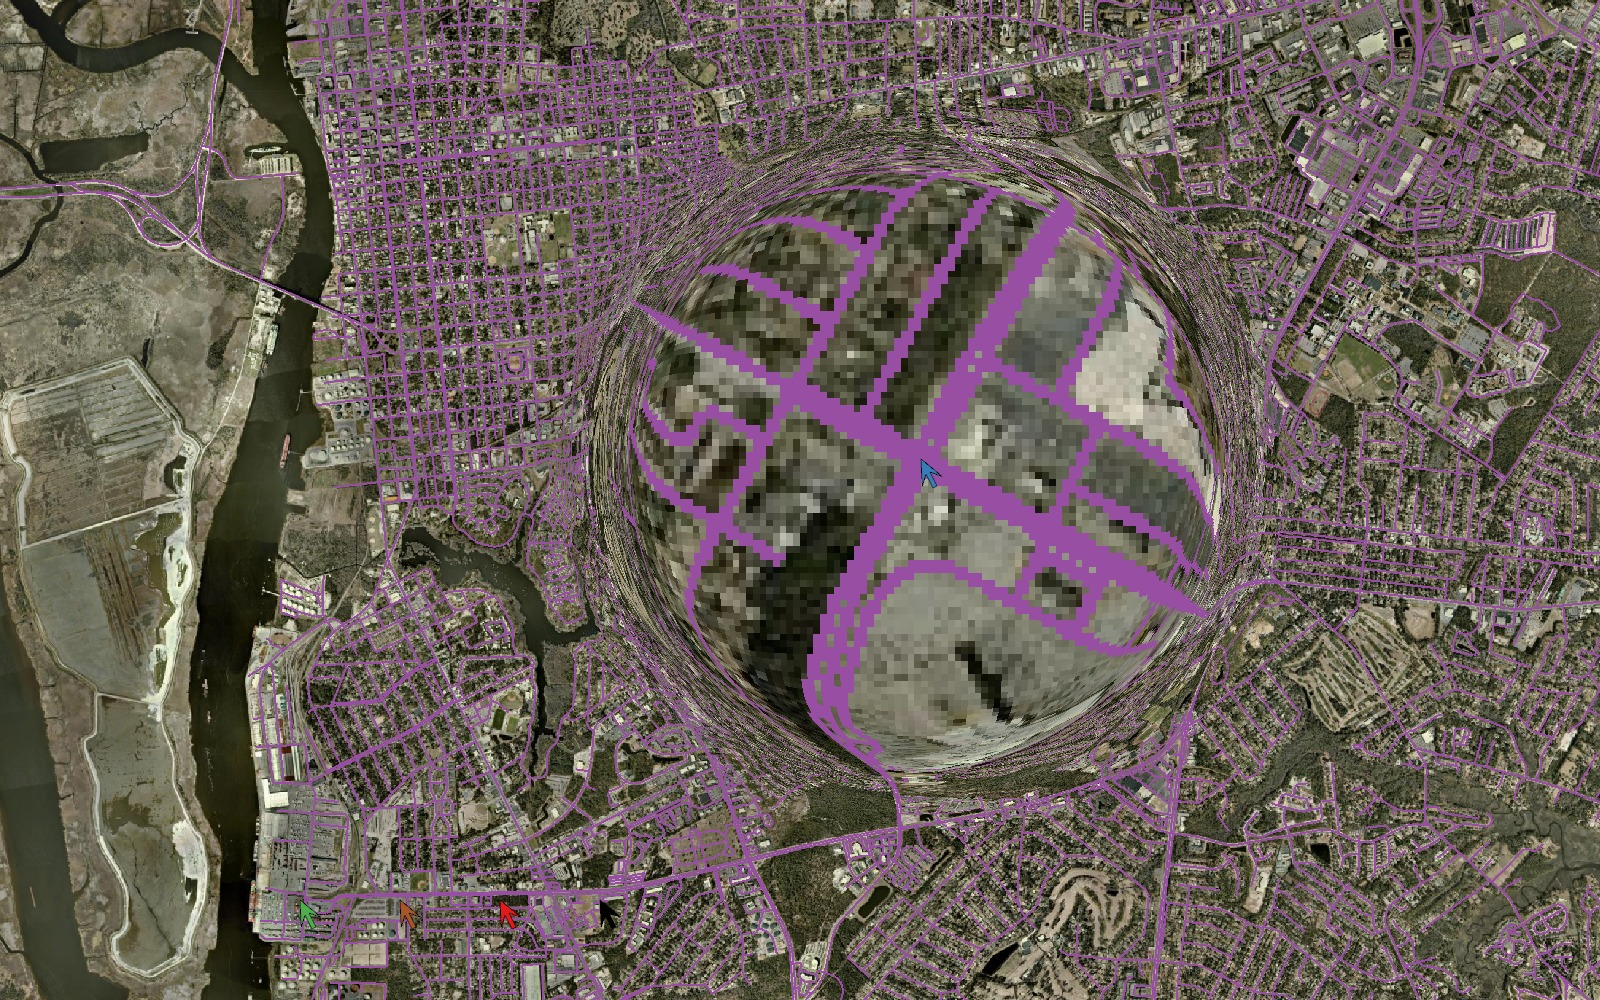
\includegraphics[width=0.49\linewidth]{img/s_r_20_zoom.jpg}
    \vspace{3 mm}

    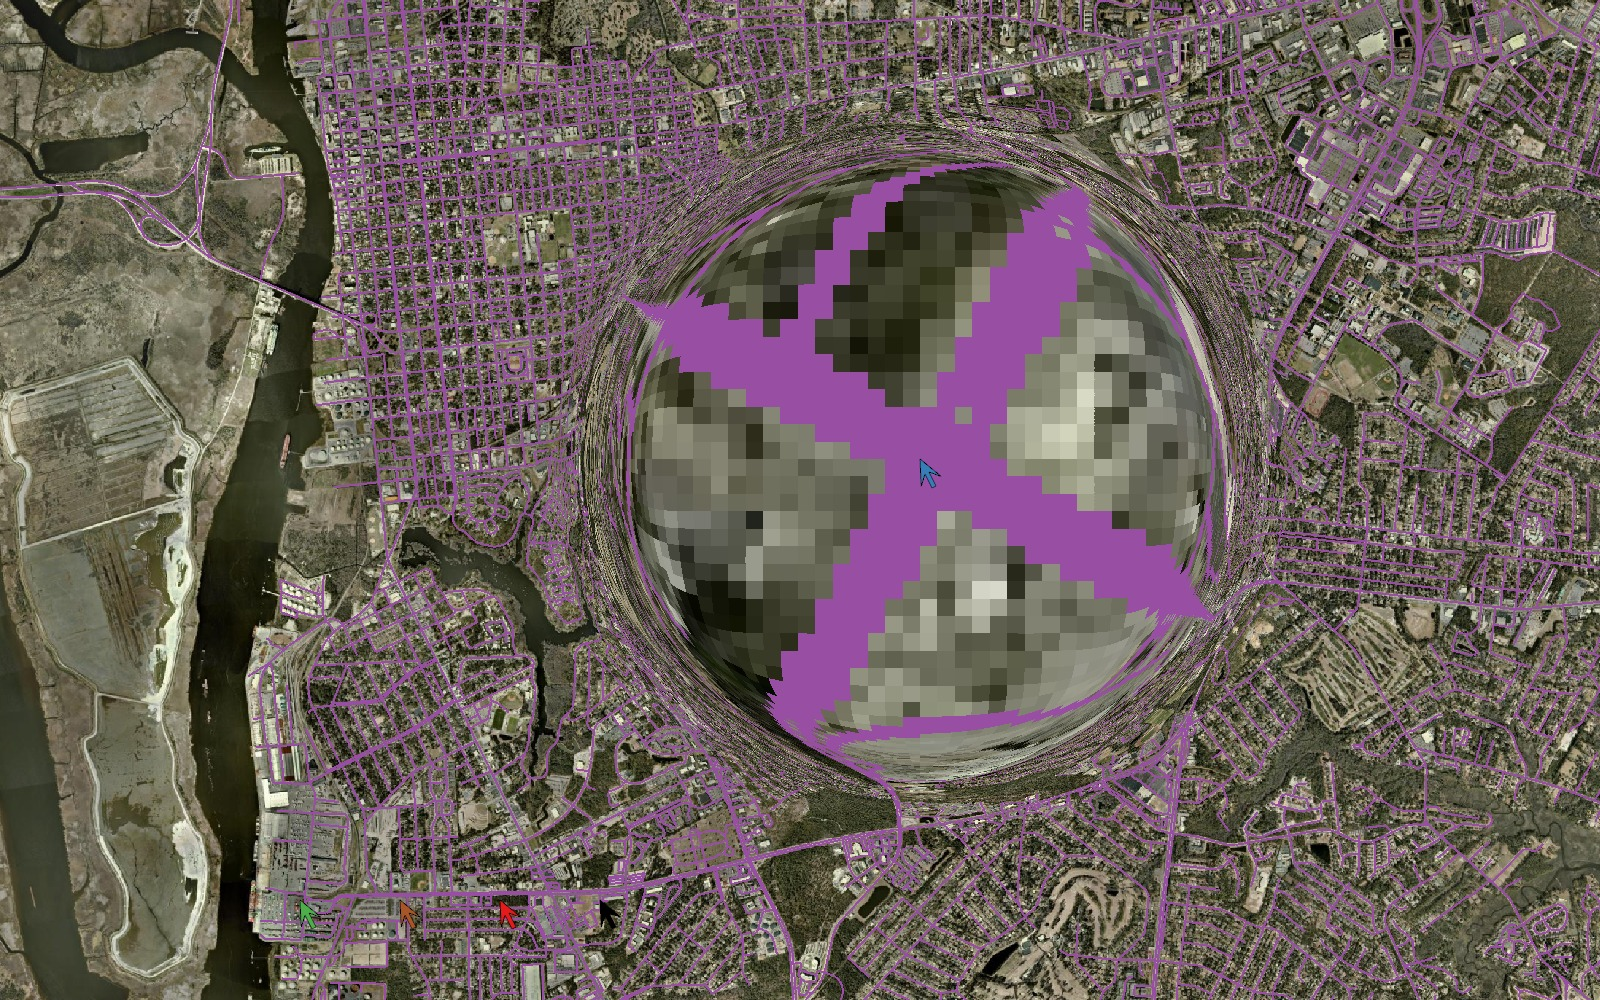
\includegraphics[width=0.49\linewidth]{img/s_r_30_zoom.jpg}
    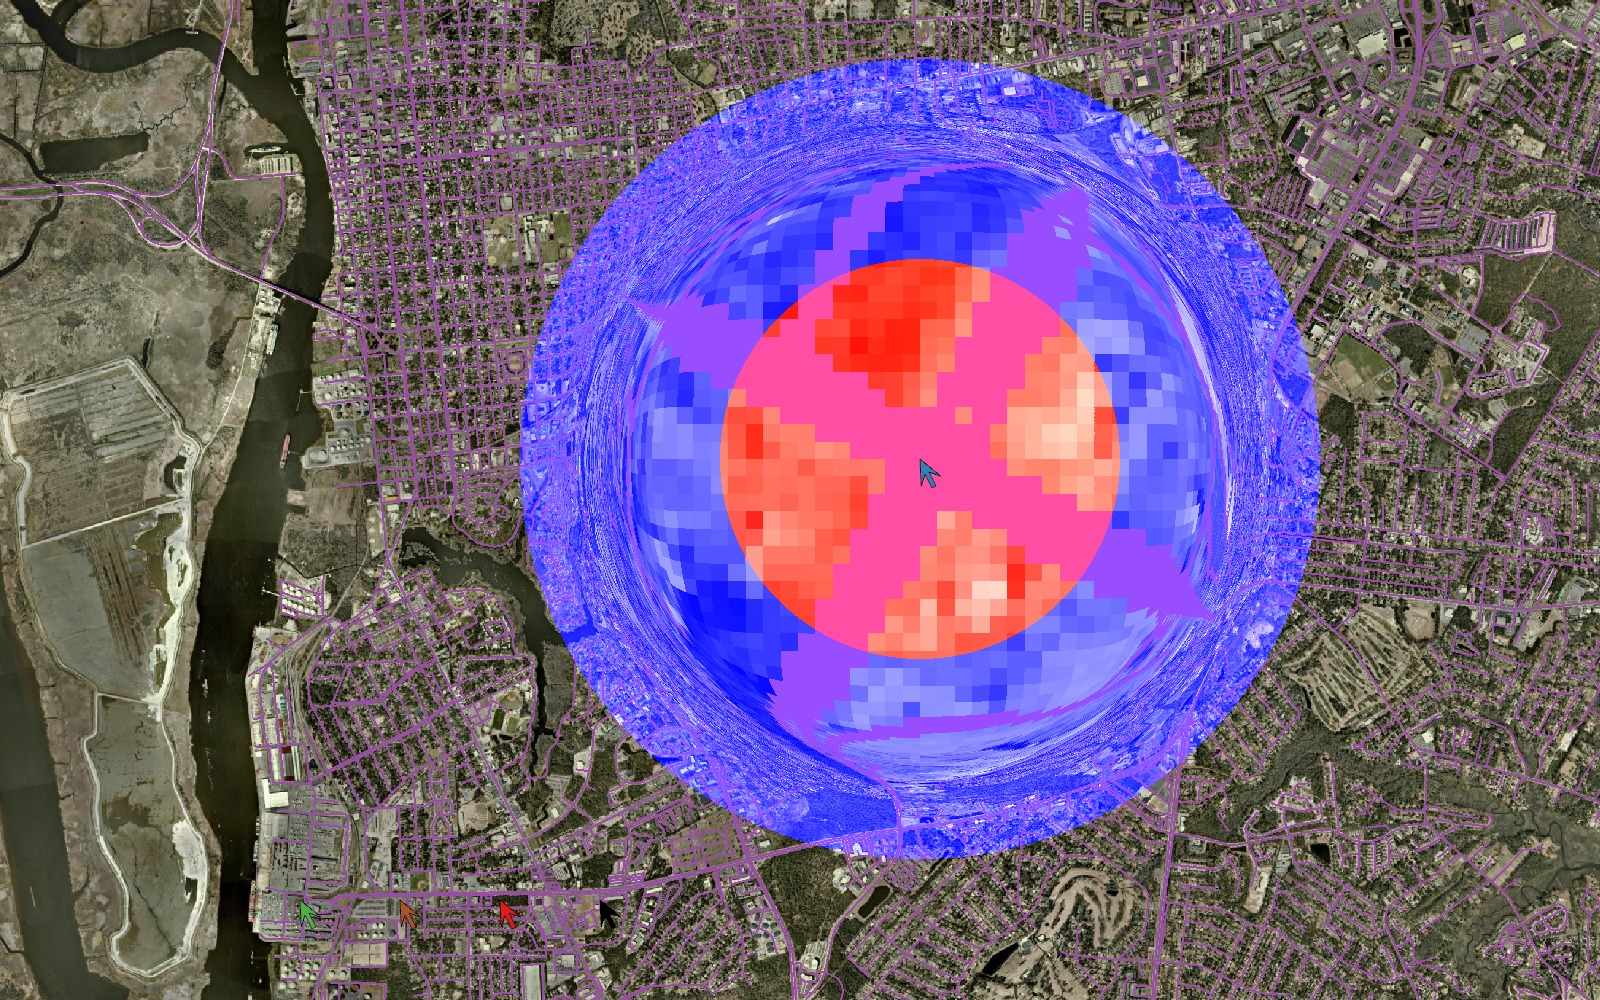
\includegraphics[width=0.49\linewidth]{img/s_r_30_zoom_color.jpg}
    \caption[Satellite Images and Road Network with 1.6x to 17.4x Linear Magnification]{This series of images 
    shows the road network and satellite images rendered at increasing levels of linear magnification, ranging 
    from 1.6x to 17.4x. Notice that the individual pixels become more noticeable as we increase the zoom. The 
    blue region represents the area of non-linear magnification, while the red region represents the area of 
    linear magnification. This is a debugging visualization for viewing the different regions of magnification.}
    \label{fig:s_r_mag}
\end{figure}

Figure~\ref{fig:s_r_g_no_zoom} shows the application without any magnification applied for a particularly dense area of graph elements. The user would like to see the individual elements separated and also see the underlying satellite imagery of the region. Figure~\ref{fig:s_r_g_mag} shows a series of images with an increasing level of linear zoom. By performing this magnification, the user is able to see the individual street and intersection information that was initially
obscured by the graph elements. As we increase the magnification of this region, the majority of the nodes become clustered in the non-linear region. Using a high magnification for these areas may end up being as detrimental as no magnification for multiple users, as the nodes are still indistinguishable from one another due to the demagnification of the blue region.

\begin{figure}[htp]\centering
    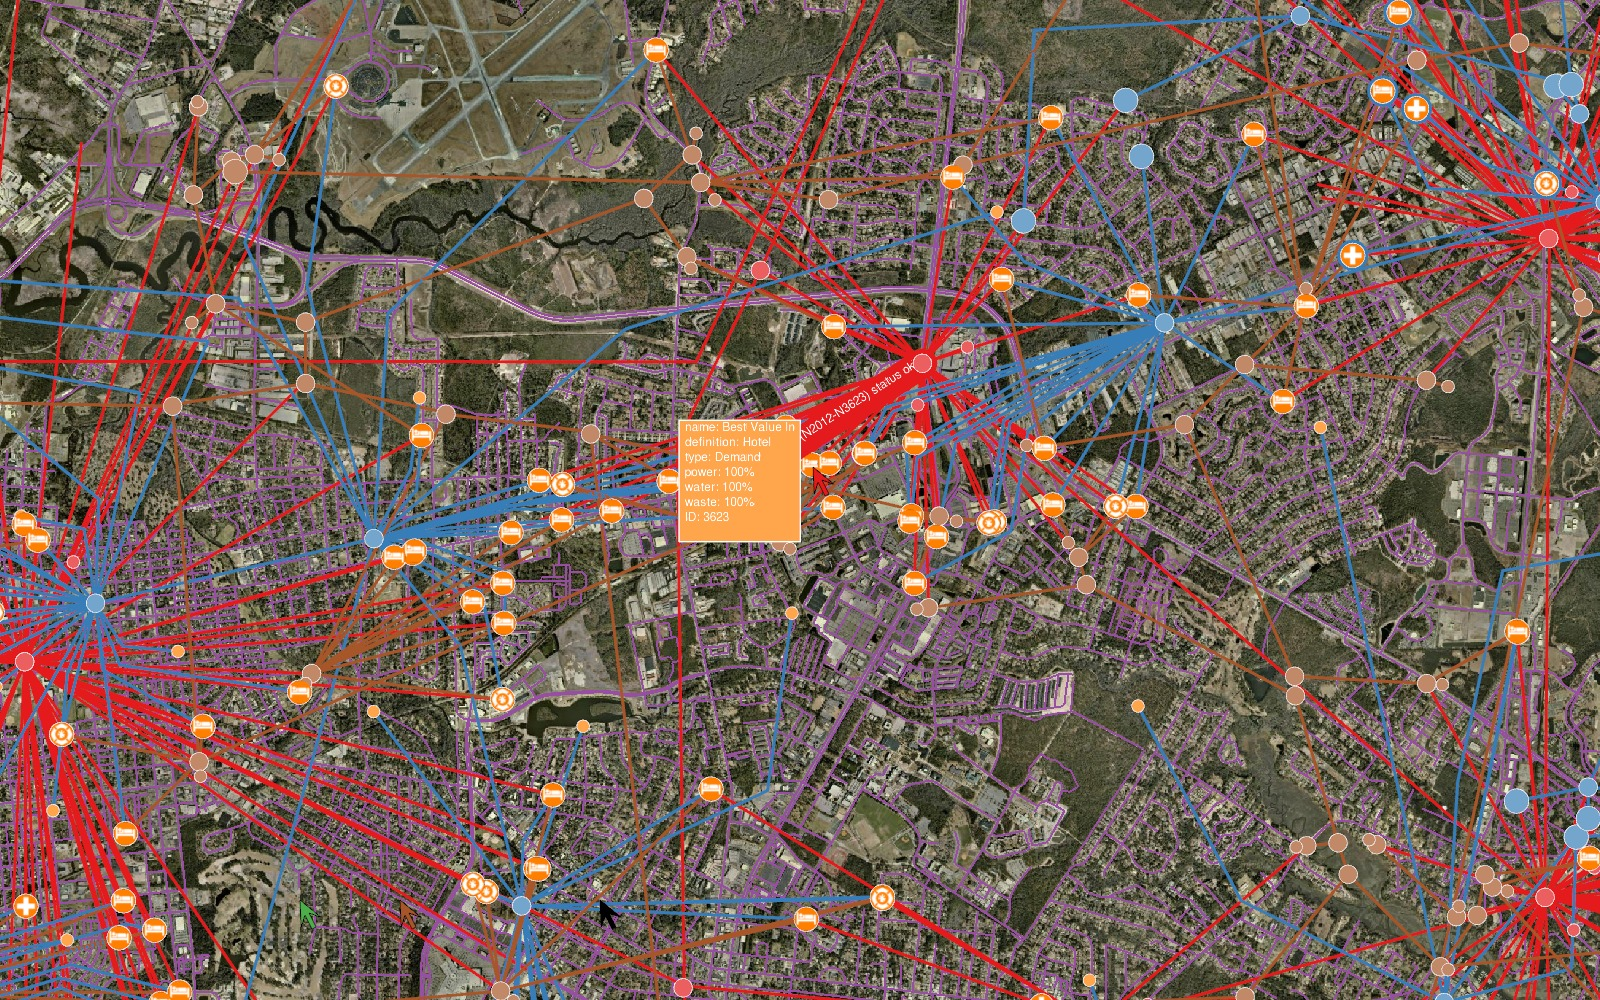
\includegraphics[width=1.0\linewidth]{img/s_r_g_no_zoom.jpg}
    \caption[Full Application without Linear Magnification]{A single image showing the application with the satellite images, graph network, and road network all displaying. This image is included as a base reference point for the images in Figure~\ref{fig:s_r_g_mag}.}
    \label{fig:s_r_g_no_zoom}
\end{figure}

\begin{figure}[htp]\centering
    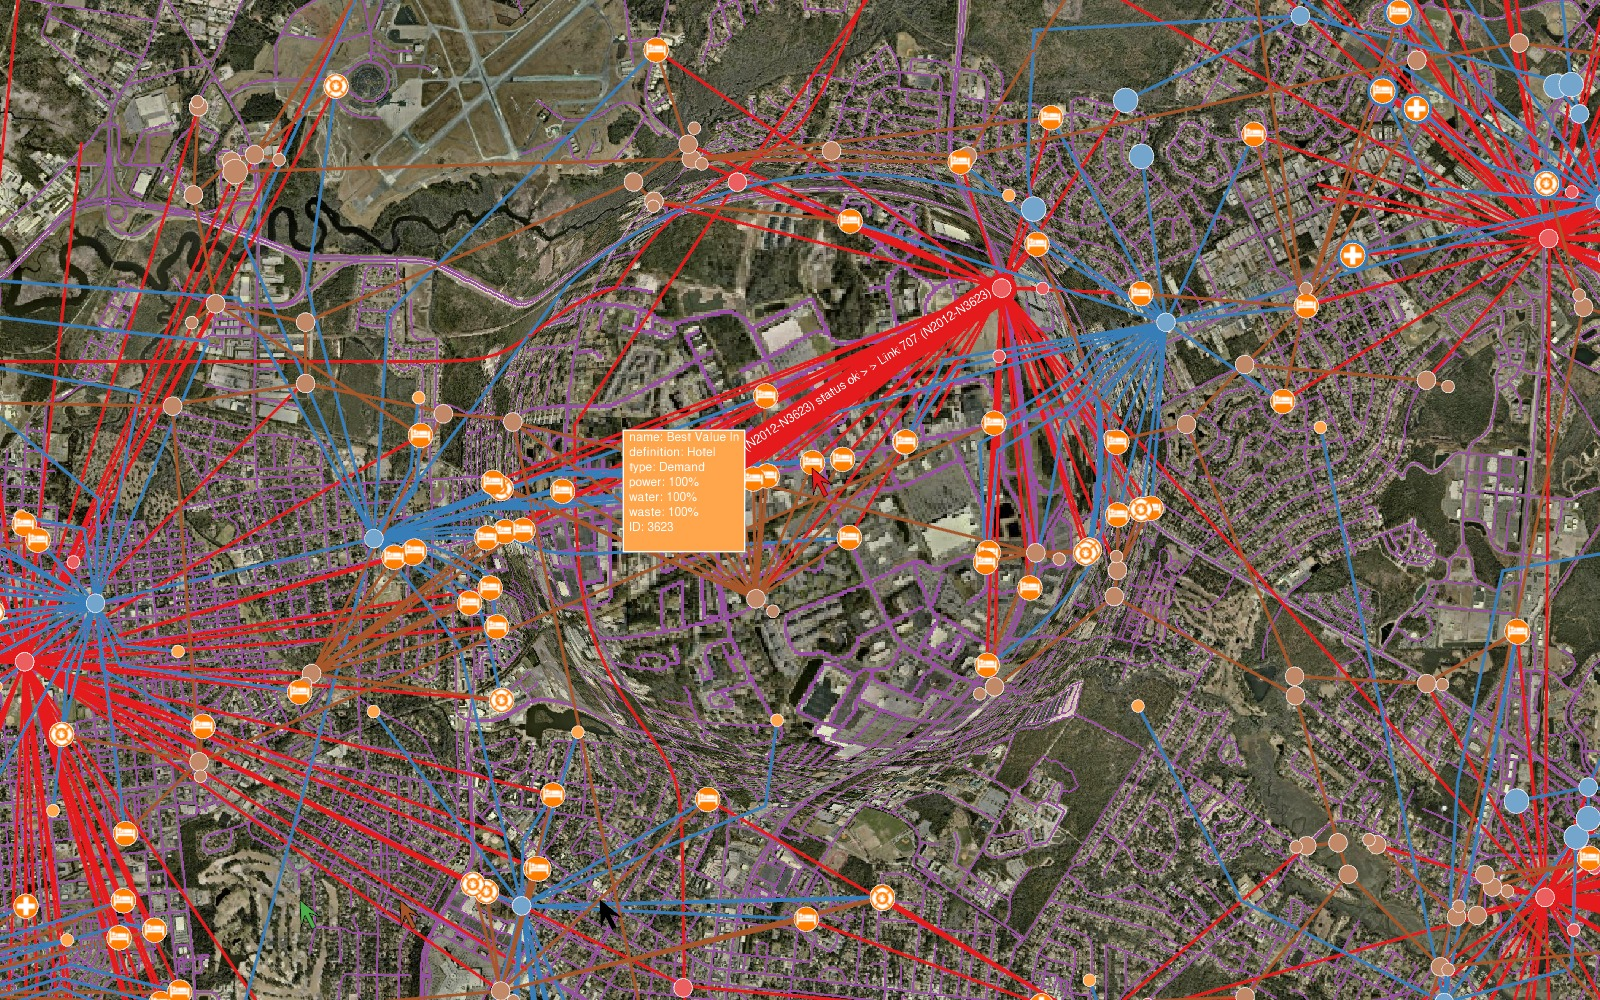
\includegraphics[width=0.49\linewidth]{img/s_r_g_5_zoom.jpg}
    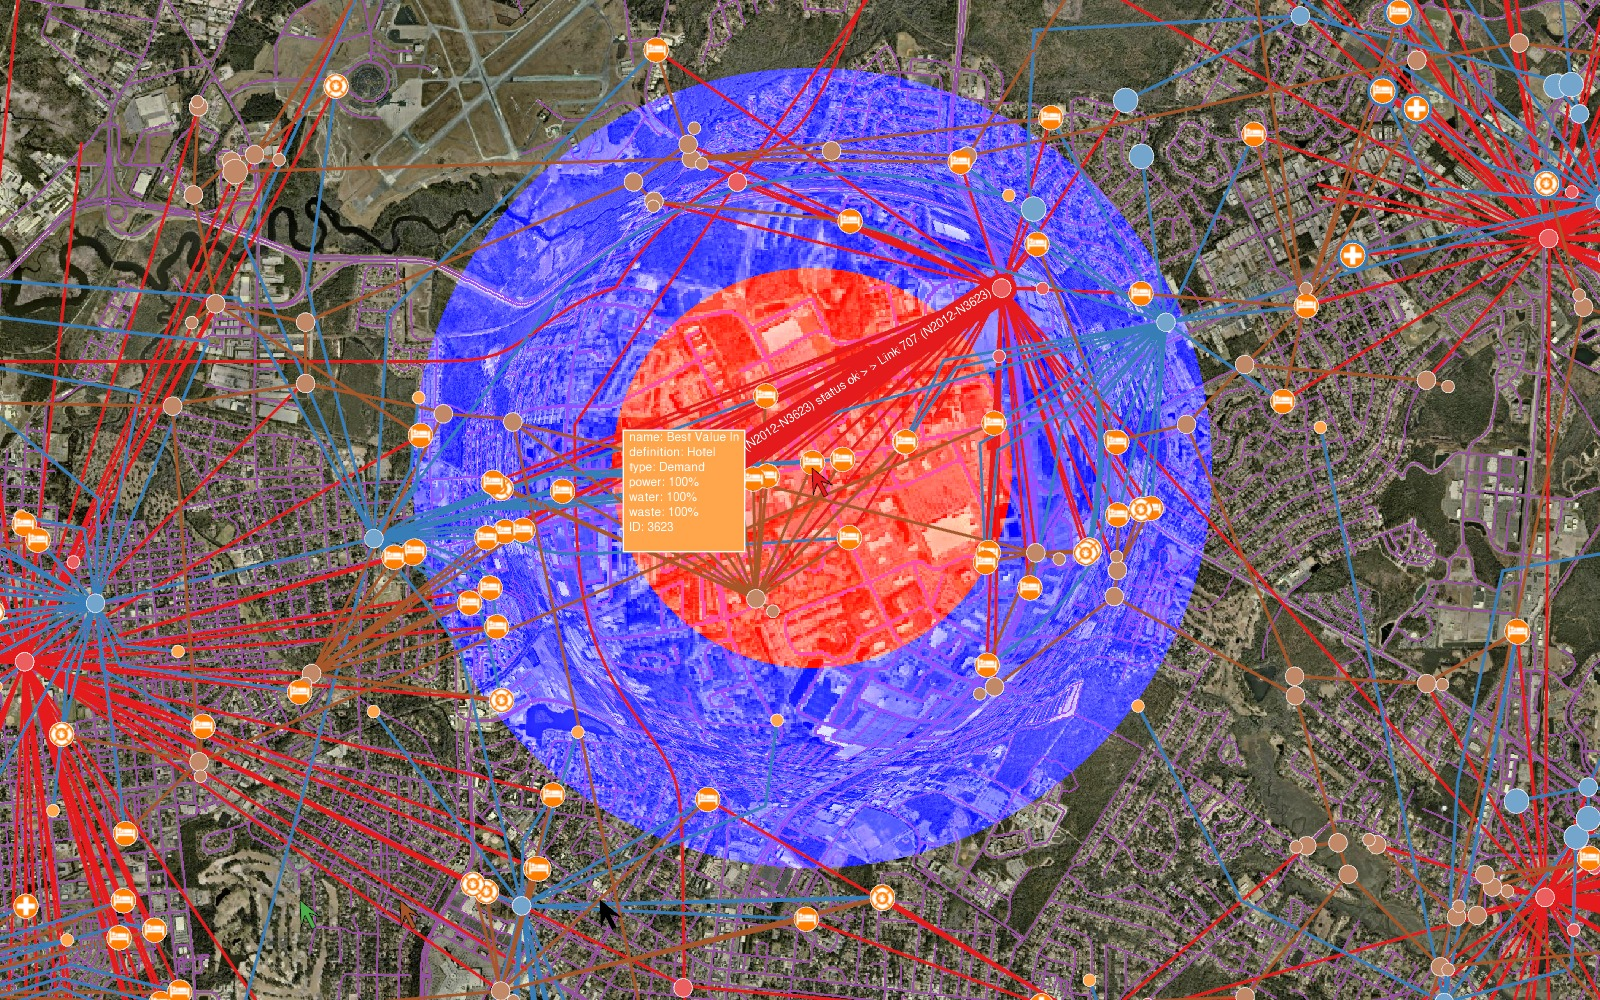
\includegraphics[width=0.49\linewidth]{img/s_r_g_5_zoom_color.jpg}
    \vspace{3 mm}

    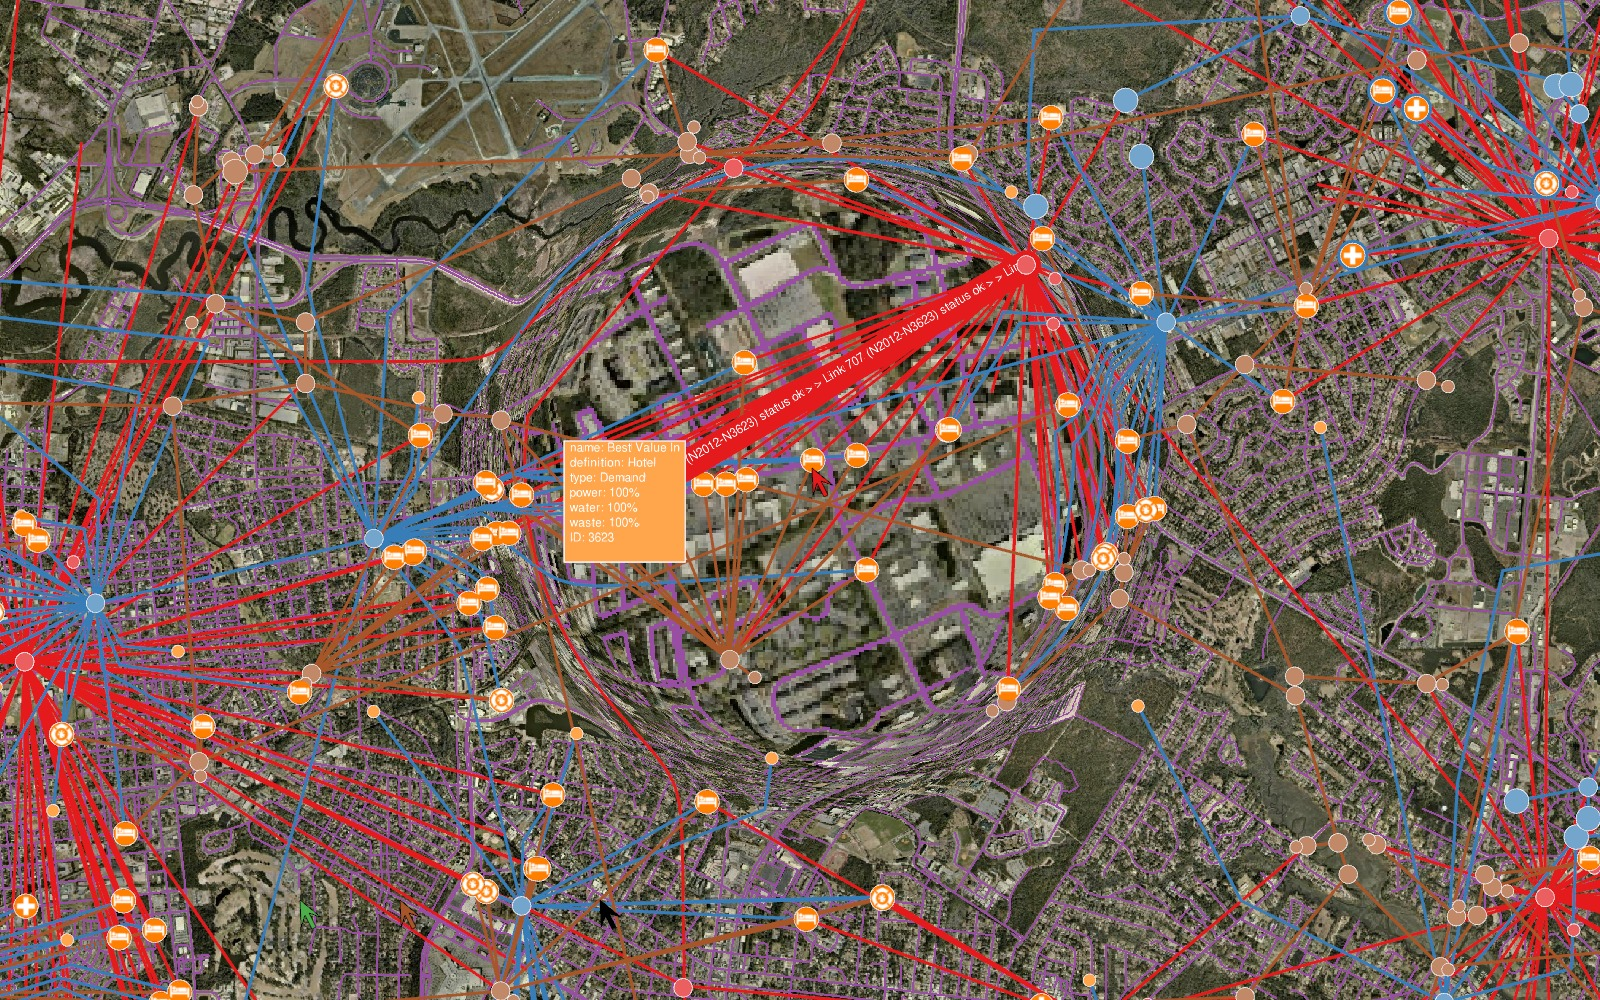
\includegraphics[width=0.49\linewidth]{img/s_r_g_10_zoom.jpg}
    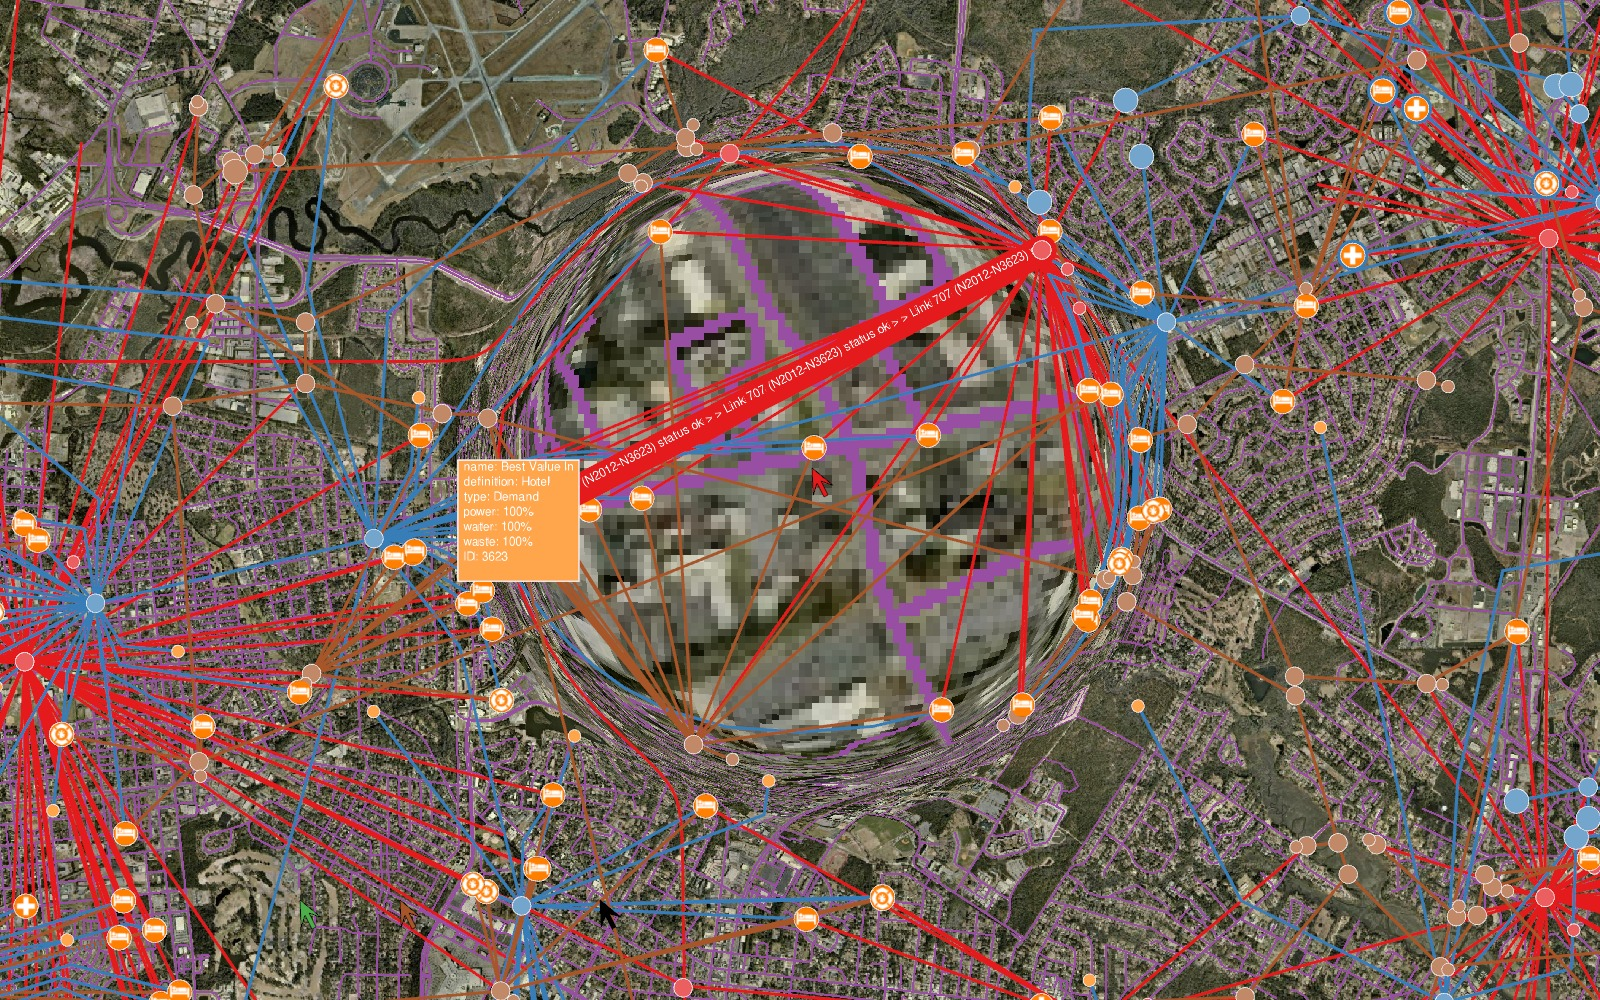
\includegraphics[width=0.49\linewidth]{img/s_r_g_20_zoom.jpg}
    \vspace{3 mm}

    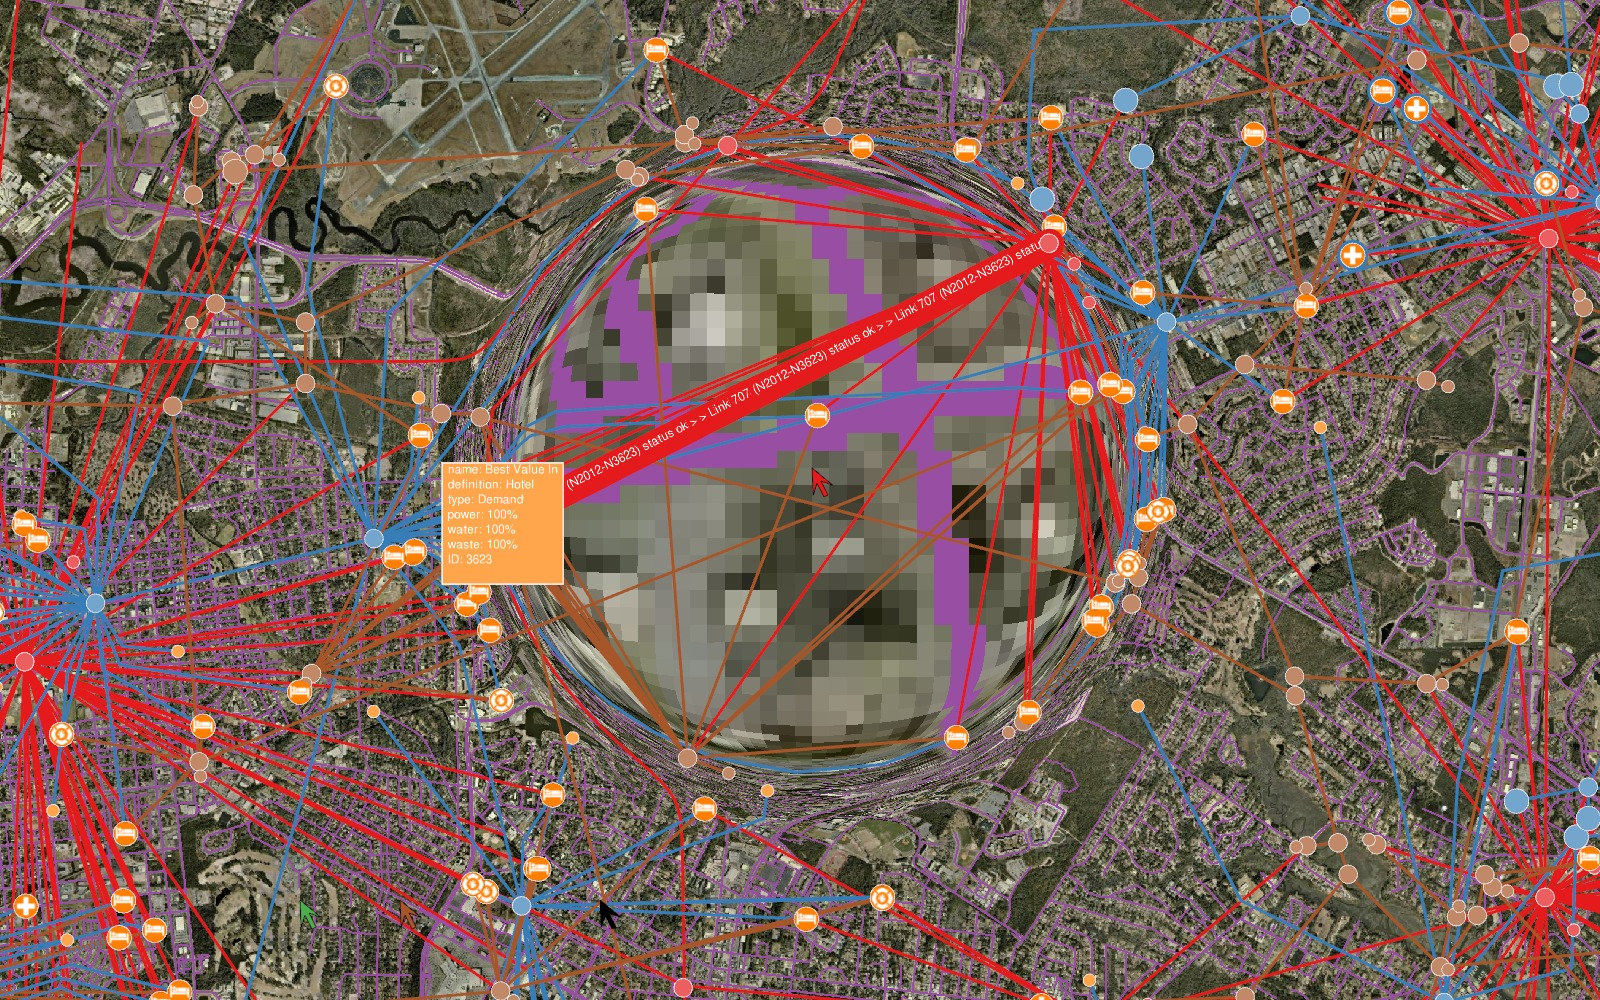
\includegraphics[width=0.49\linewidth]{img/s_r_g_30_zoom.jpg}
    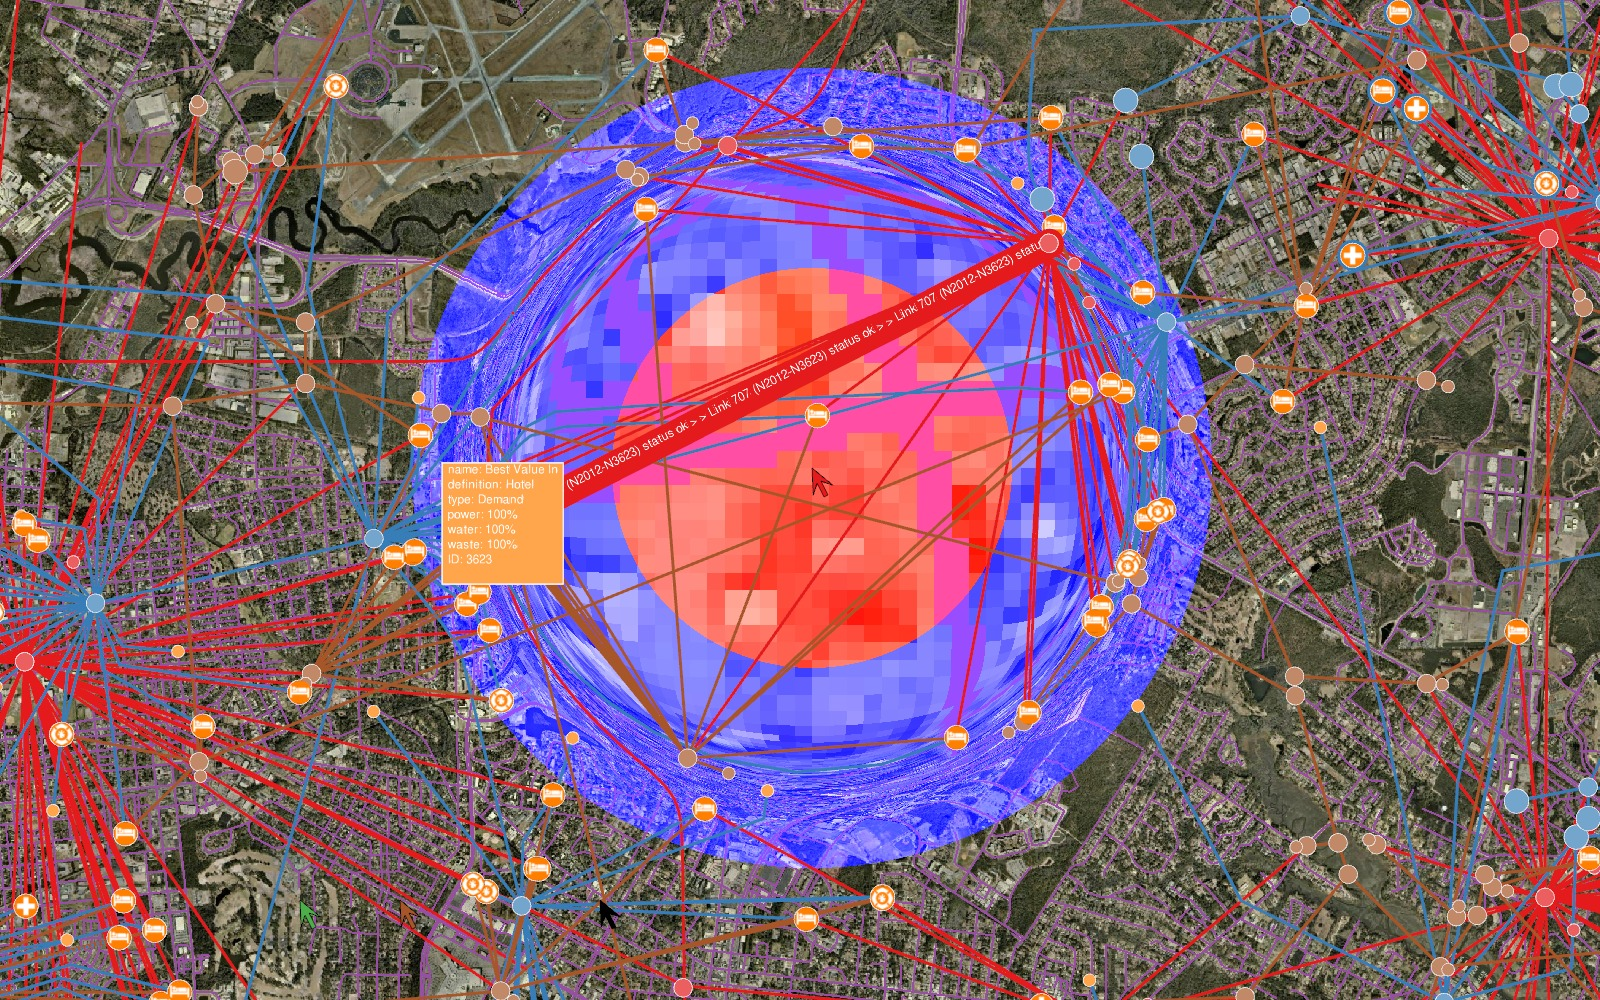
\includegraphics[width=0.49\linewidth]{img/s_r_g_30_zoom_color.jpg}
    \caption[Full Application with 1.6x to 17.4x Linear Magnification]{These images show the full application with an increasing level of linear magnification affecting both the graph data and the satellite images. The user is currently diagnosing a problem with the group of hotels in this region.}
    \label{fig:s_r_g_mag}
\end{figure}

The interaction between multiple magnification areas is seen in Figure~\ref{fig:problem_solving}. Both users are diagnosing a problem in the same area, and are able to see the region around their cursors in greater detail without affecting the other user. Note that the river between the two sites is still clearly visible, along with the edges between elements for both regions. This functionality allows the individual users to still see the relationship between their specific graph
elements to the overall system, further assisting in diagnosing the problems within the region.

\begin{figure}[htp]\centering
    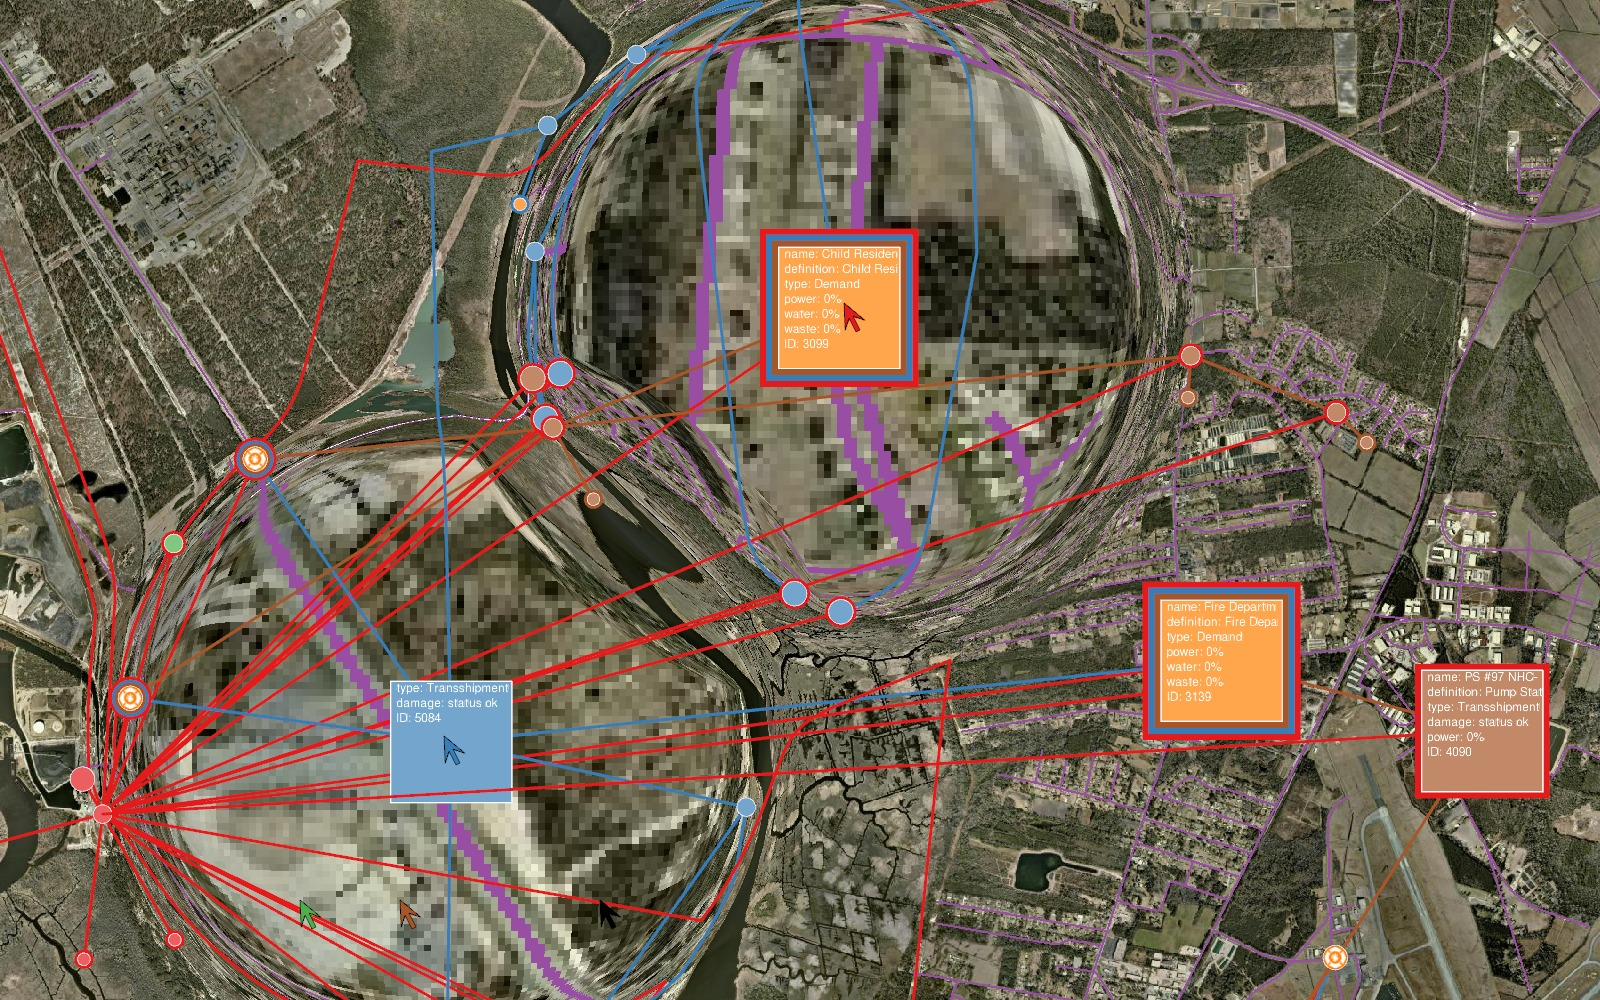
\includegraphics[width=0.49\linewidth]{img/problem_solving_20_20.jpg}
    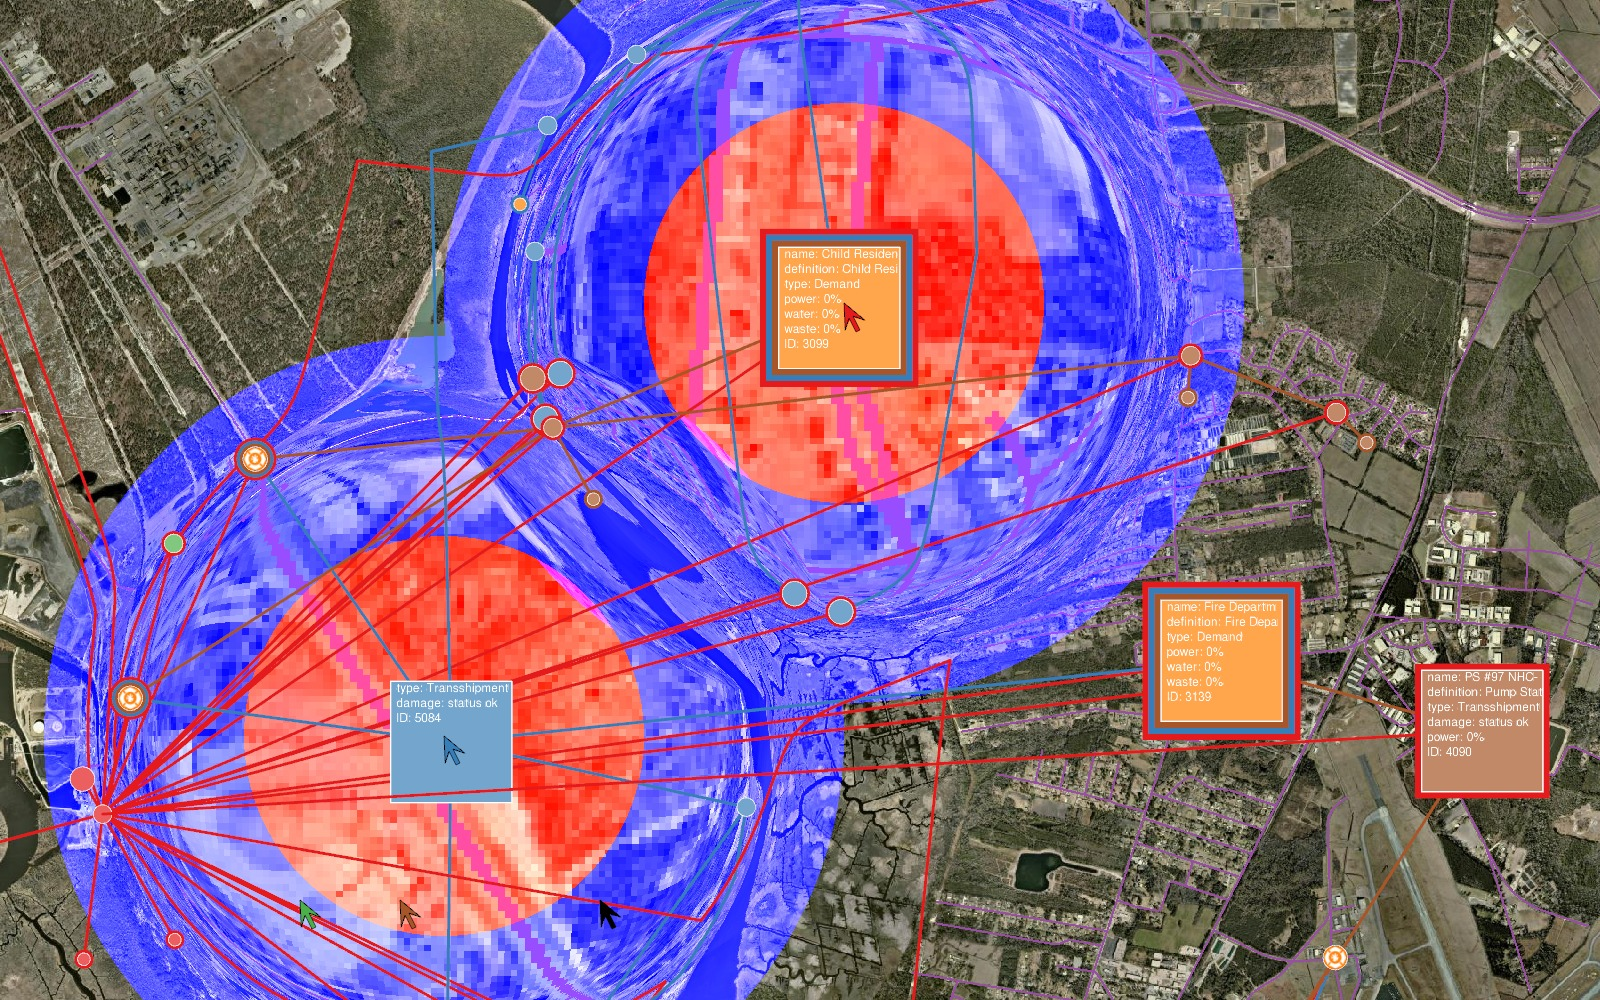
\includegraphics[width=0.49\linewidth]{img/problem_solving_20_20_color.jpg}
    \caption[Full Application with Two Areas of 6.7x Colored Linear Magnification]{An image showing the combined areas of magnification between two cursors. Each user is able to see their own region of interest in greater detail.}
    \label{fig:problem_solving}
\end{figure}

\begin{figure}[htp]\centering
    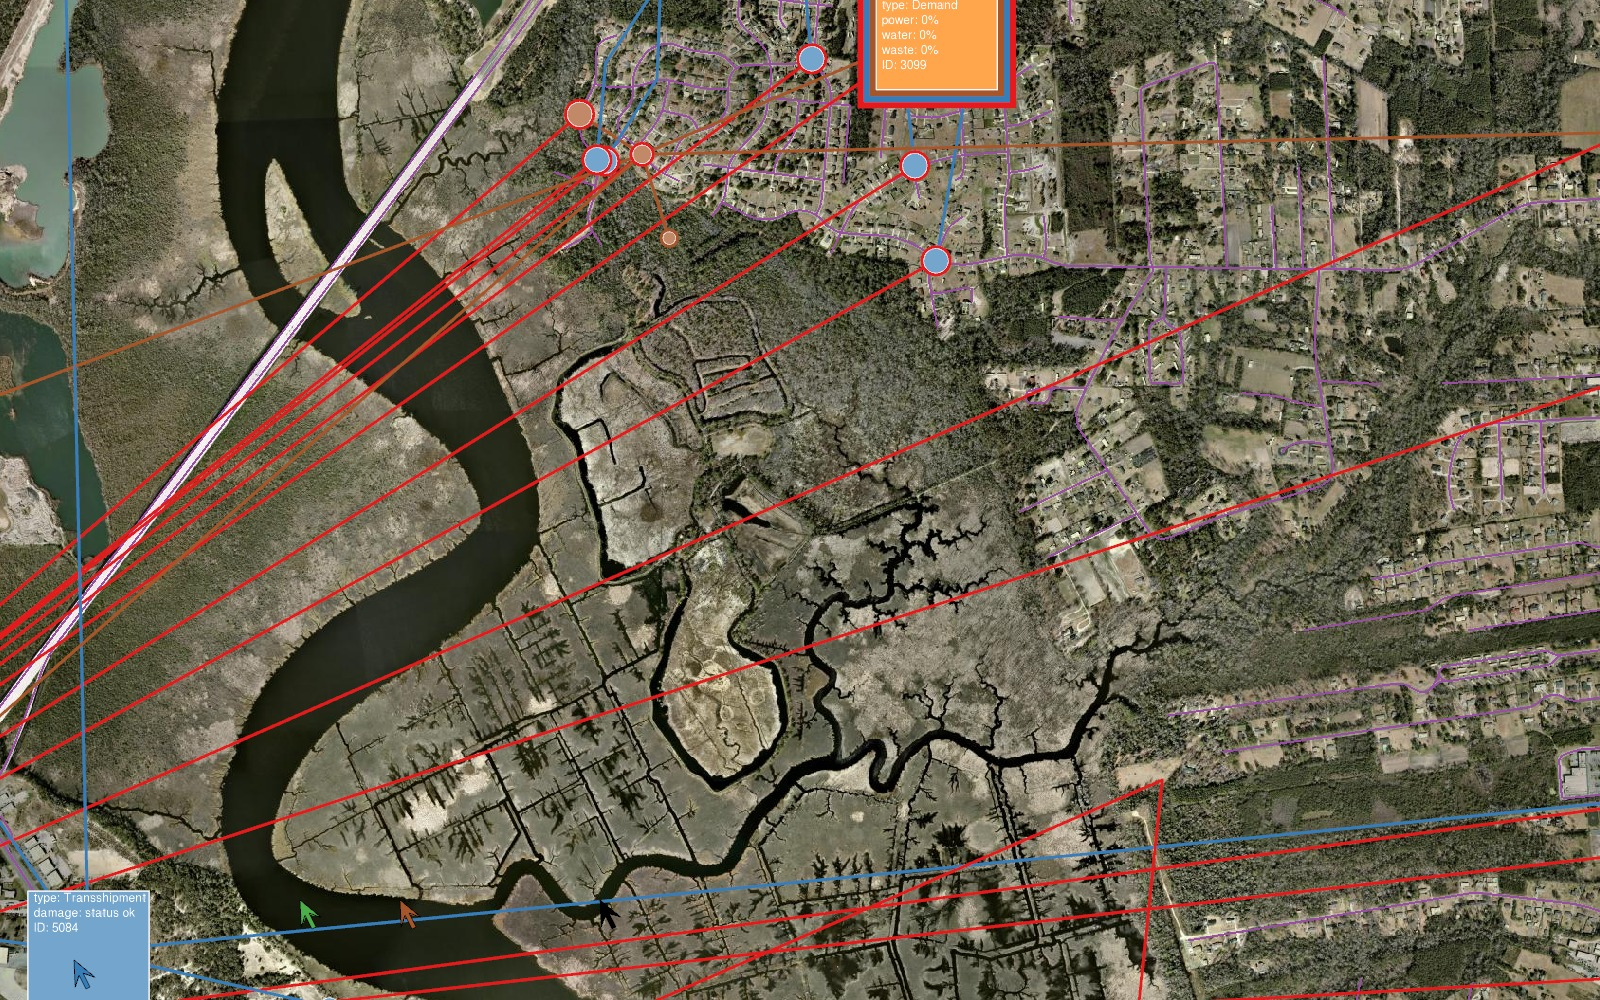
\includegraphics[width=0.90\linewidth]{img/normal_zoom.jpg}
    \caption[Full Application with Global Magnification]{The same nodes seen in Figure~\ref{fig:problem_solving}, with the maximum global magnification applied which has both nodes on screen. We cannot see the same level of local satellite imagery near the end points in question. }
    \label{fig:old_problem_solving}
\end{figure}

We can compare the focus plus context magnification seen in Figure~\ref{fig:problem_solving} to the global magnification seen in Figure~\ref{fig:old_problem_solving}. It is immediately apparent that the global magnification does not provide the same level in any way when compared to the focus plus context results. Many graph elements are now missing from this picture due to the global zoom, so it is difficult to see how these two nodes relate to other nodes within the graph.
This global magnification also fails to adequately show much geographic information about the area surrounding each of the expanded nodes.


Figure~\ref{fig:centered} shows a single cursor interacting with a single graph node and edge. If we examine the magnification of the satellite images and graph network, we can see that the node stays in the same geographic location, i.e.\ if this was a physical map, the node stays stuck to its position even when we fold the map to produce a magnification. This was the intended purpose of the magnification for both the satellite images and graph network, as it allows for users to see high magnification satellite data and interact with the system without performing a global
zoom. Unfortunately, because the nodes remain geographically rooted, interacting with graph elements becomes more difficult. The cursor still moves in screen space, despite covering more geographic space. The elements also move from their original position, requiring more hand-eye coordination to accurately interact with the elements. This problem is further exacerbated when higher levels of magnification are used, as the elements simply move around a cursor even faster.

\begin{figure}[htp]\centering
    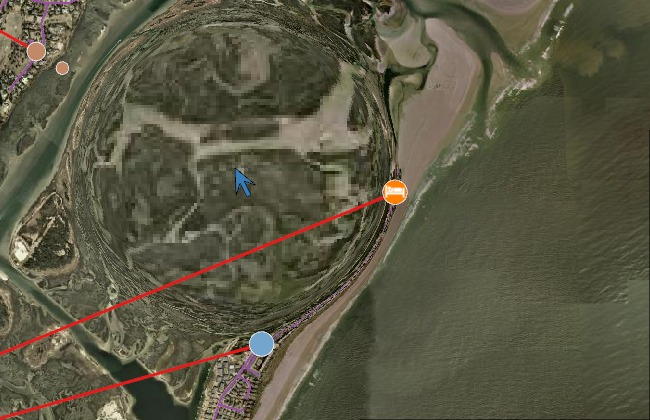
\includegraphics[width=0.40\linewidth]{img/12_edge_crop.jpg}
    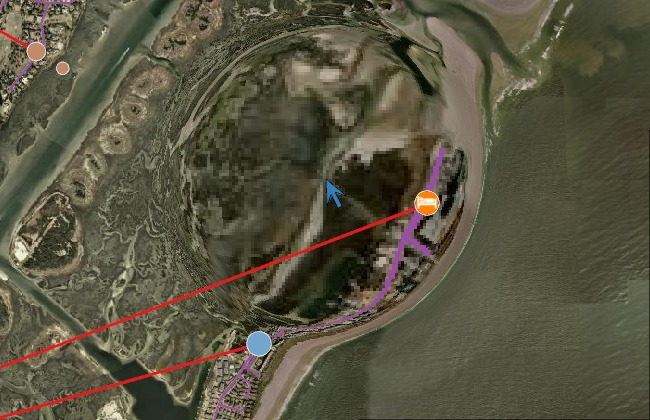
\includegraphics[width=0.40\linewidth]{img/12_mild_offset_crop.jpg}
    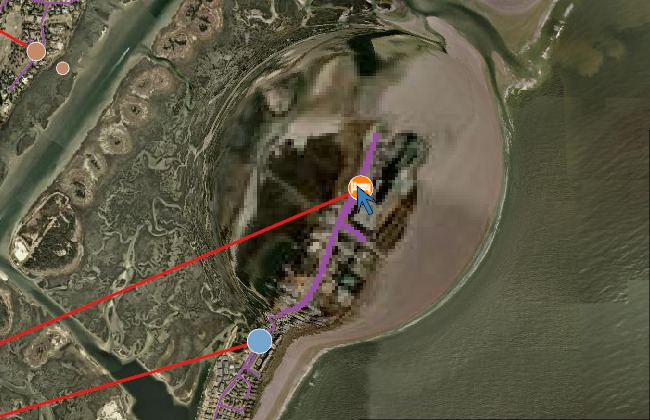
\includegraphics[width=0.40\linewidth]{img/12_center_crop.jpg}
    \caption[Node and Satellite Image Interaction with 3.1x Linear Magnification Centered on Node]{These images depict a single cursor trying to center itself on a particular node. There is some slight difficulty in this task, as the node changes position due to the magnification function. Currently, the cursor movement is relative to the original unmagnified screenspace, so with high magnification, the movement of the cursor is visually fast in the magnified region.}
    \label{fig:centered}
\end{figure}

\begin{figure}[htp]\centering
    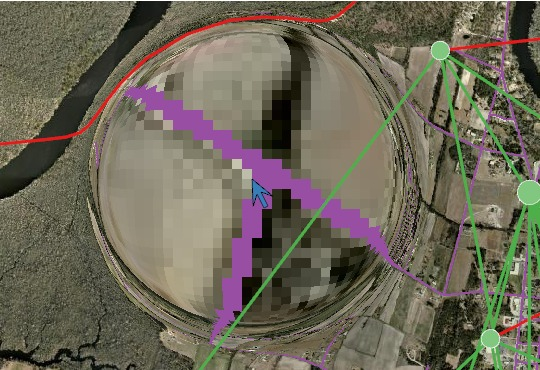
\includegraphics[width=0.90\linewidth]{img/p_vs_t_clip.jpg}
    \caption[Edge Differences]{An image showing that edges which have a defined path, such as red buried power lines, retain their geographic location during magnification and bend around the magnification region. This contrasts with the green communication edge which connects nodes with a straight line regardless of the magnification. }
    \label{fig:edge_differences}
\end{figure}

Certain edges within the system are defined to follow a specific path. These edges were subdivided into many smaller line segments to have the shape of the path retain its geographic location when magnified. This subdivision occurred on edges which were defined with more than two end points. This was simply a rough proof of concept, and can easily be extended to look for details within the edges themselves to perform this subdivision. An image displaying the visualization of two different
edges is seen in Figure~\ref{fig:edge_differences}. 

Finally, Figure~\ref{fig:ratio} shows the flexibility of the generated magnification functions for the application. As we increase the size of the linear magnification, the region of non-linear data becomes more distorted, resulting in data loss. When the linear and non-linear regions are the same size, we see that the satellite images and road network lose data completely, as the magnification function is no longer C0 continuous. The image with mostly linear magnification
but a slight amount of non-linear seems to provide the most benefit, as the data within the linear region is undistorted, and the global context of the data is still mostly retained.


\begin{figure}[htp]\centering
    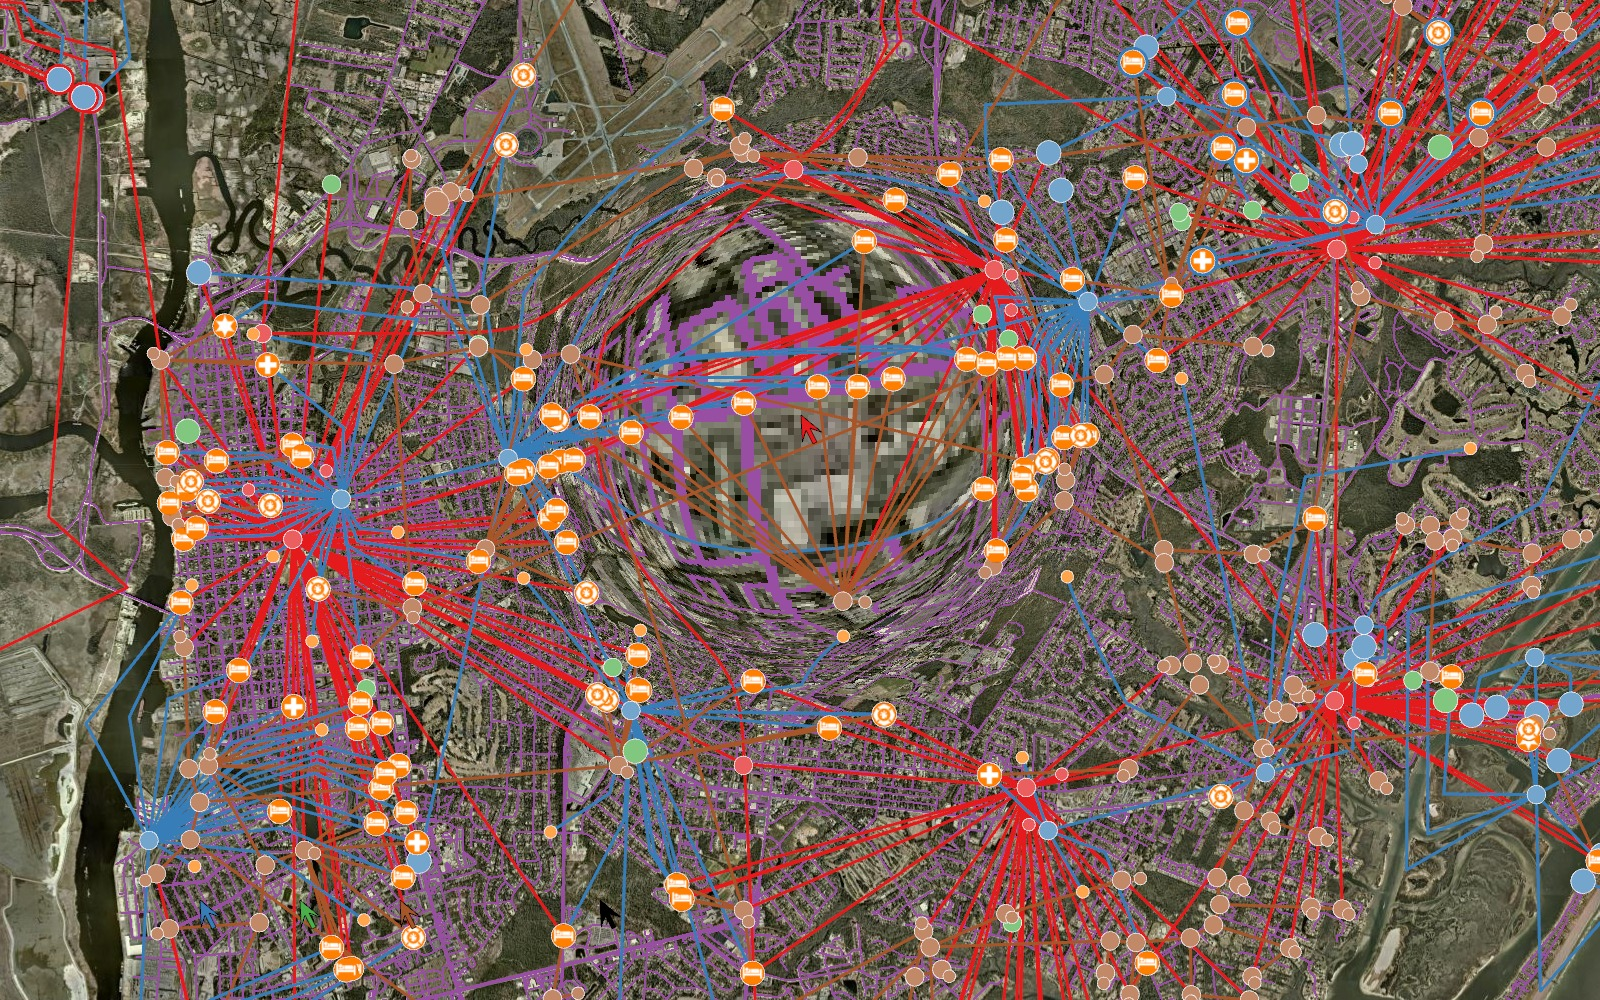
\includegraphics[width=0.40\linewidth]{img/20_no_linear.jpg}
    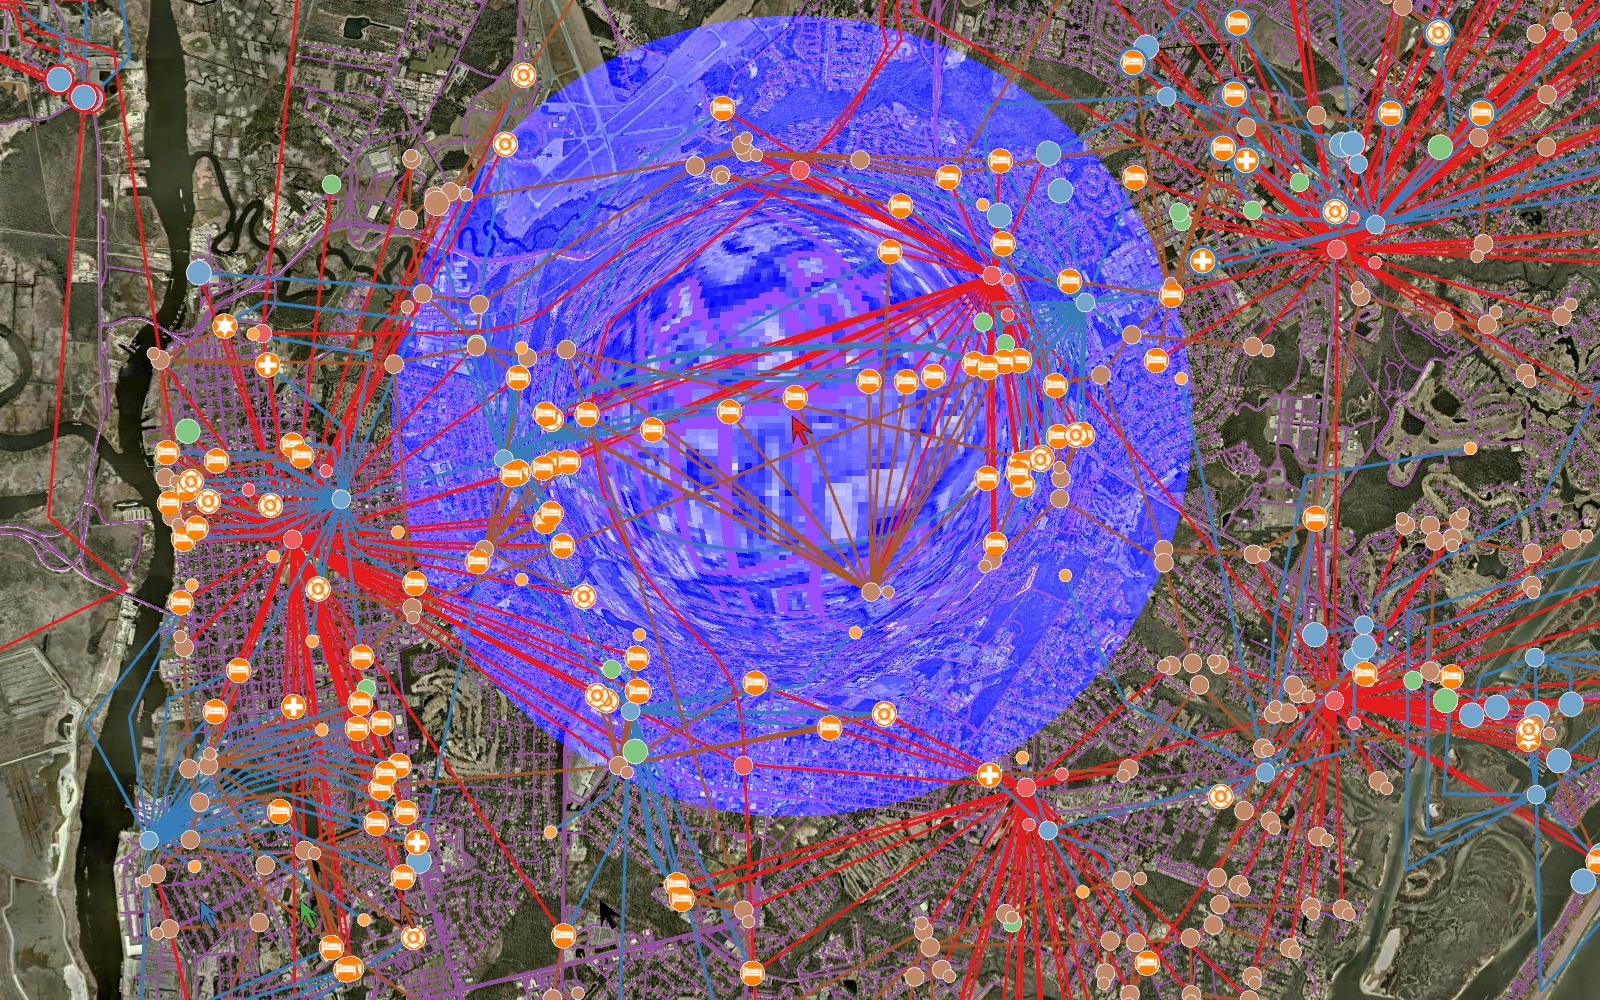
\includegraphics[width=0.40\linewidth]{img/20_no_linear_color.jpg}
    \vspace{3 mm}
    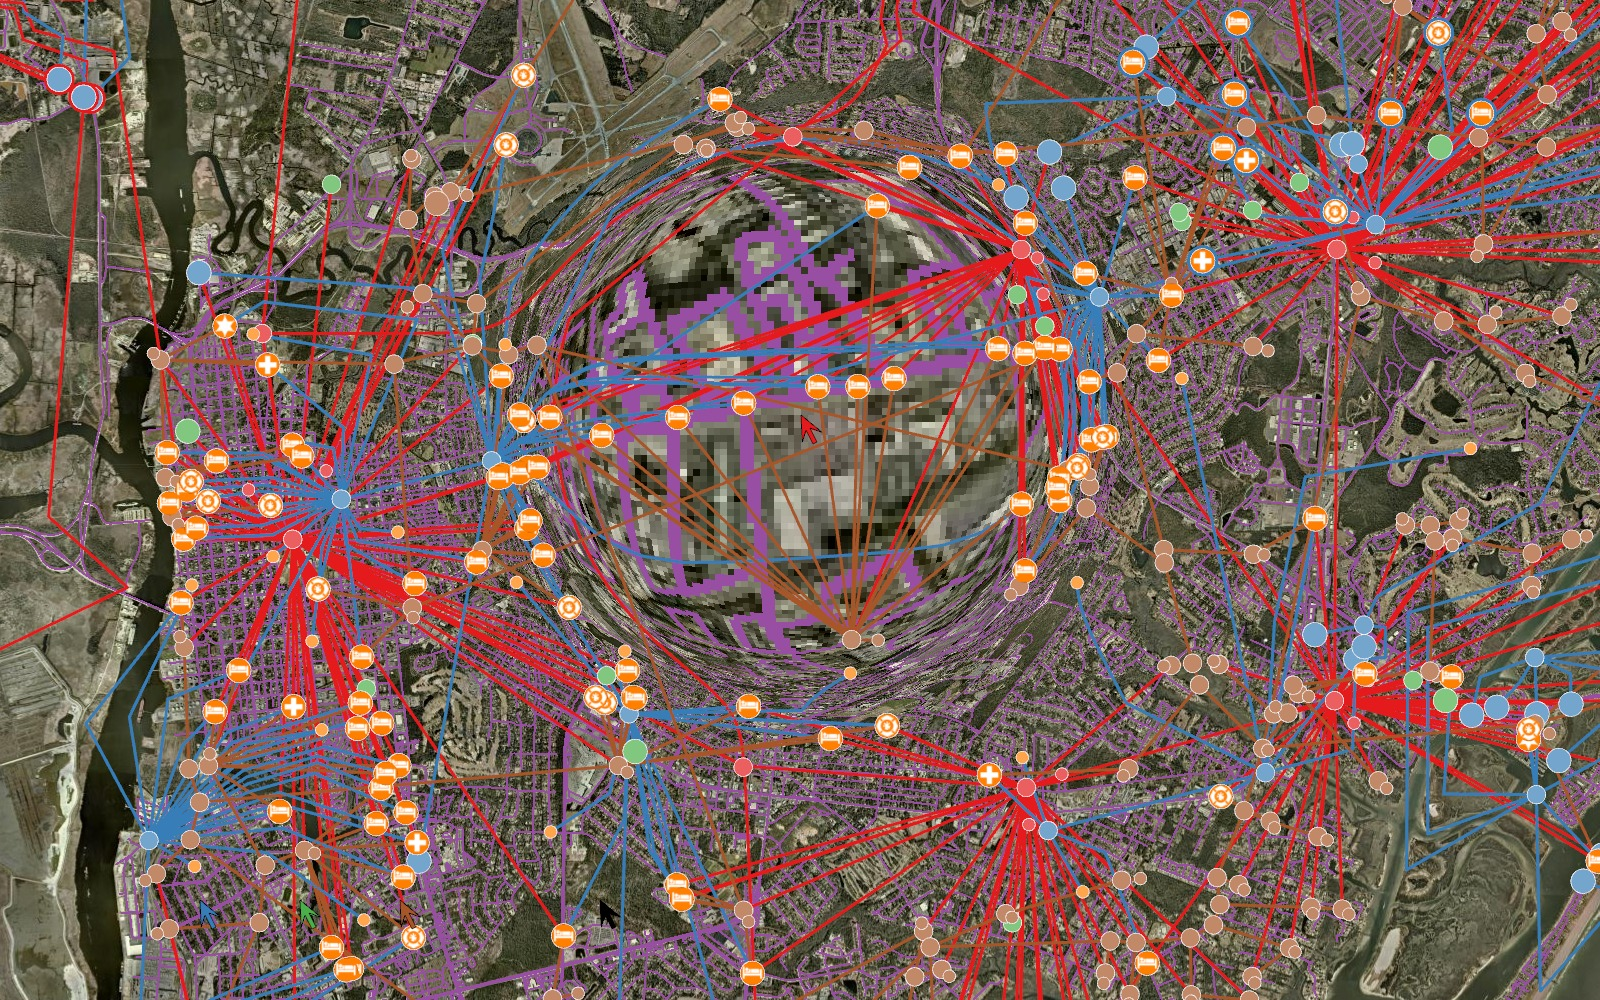
\includegraphics[width=0.40\linewidth]{img/20_one_quarter.jpg}
    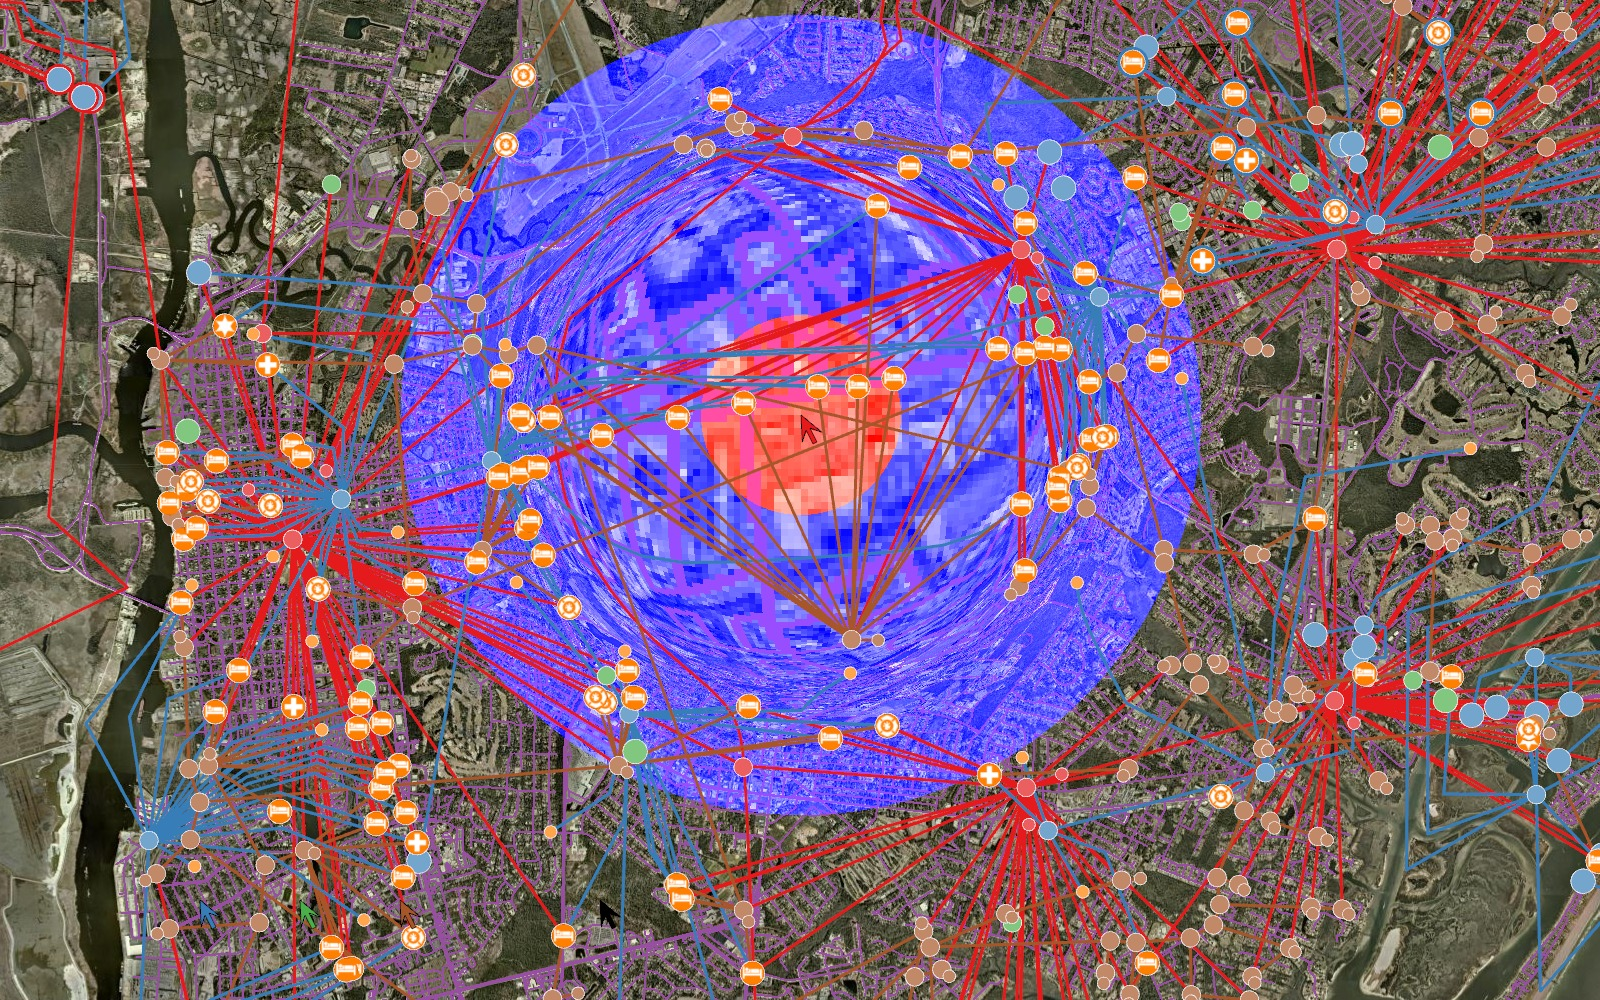
\includegraphics[width=0.40\linewidth]{img/20_one_quarter_color.jpg}
    \vspace{3 mm}
    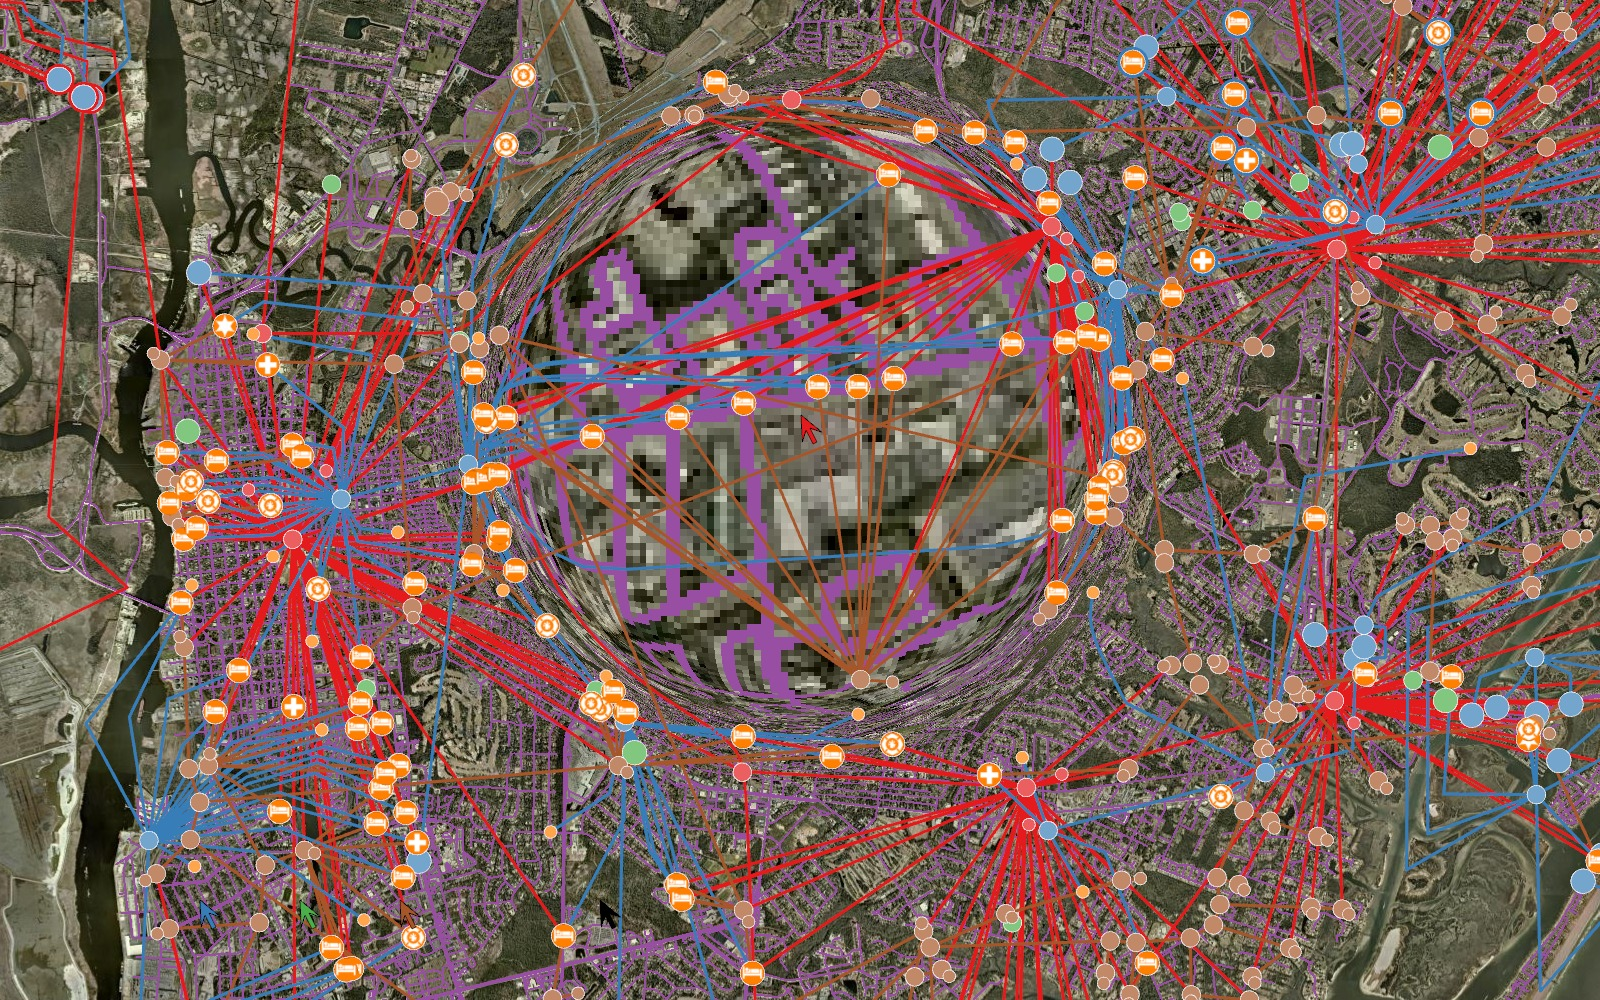
\includegraphics[width=0.40\linewidth]{img/20_half_linear.jpg}
    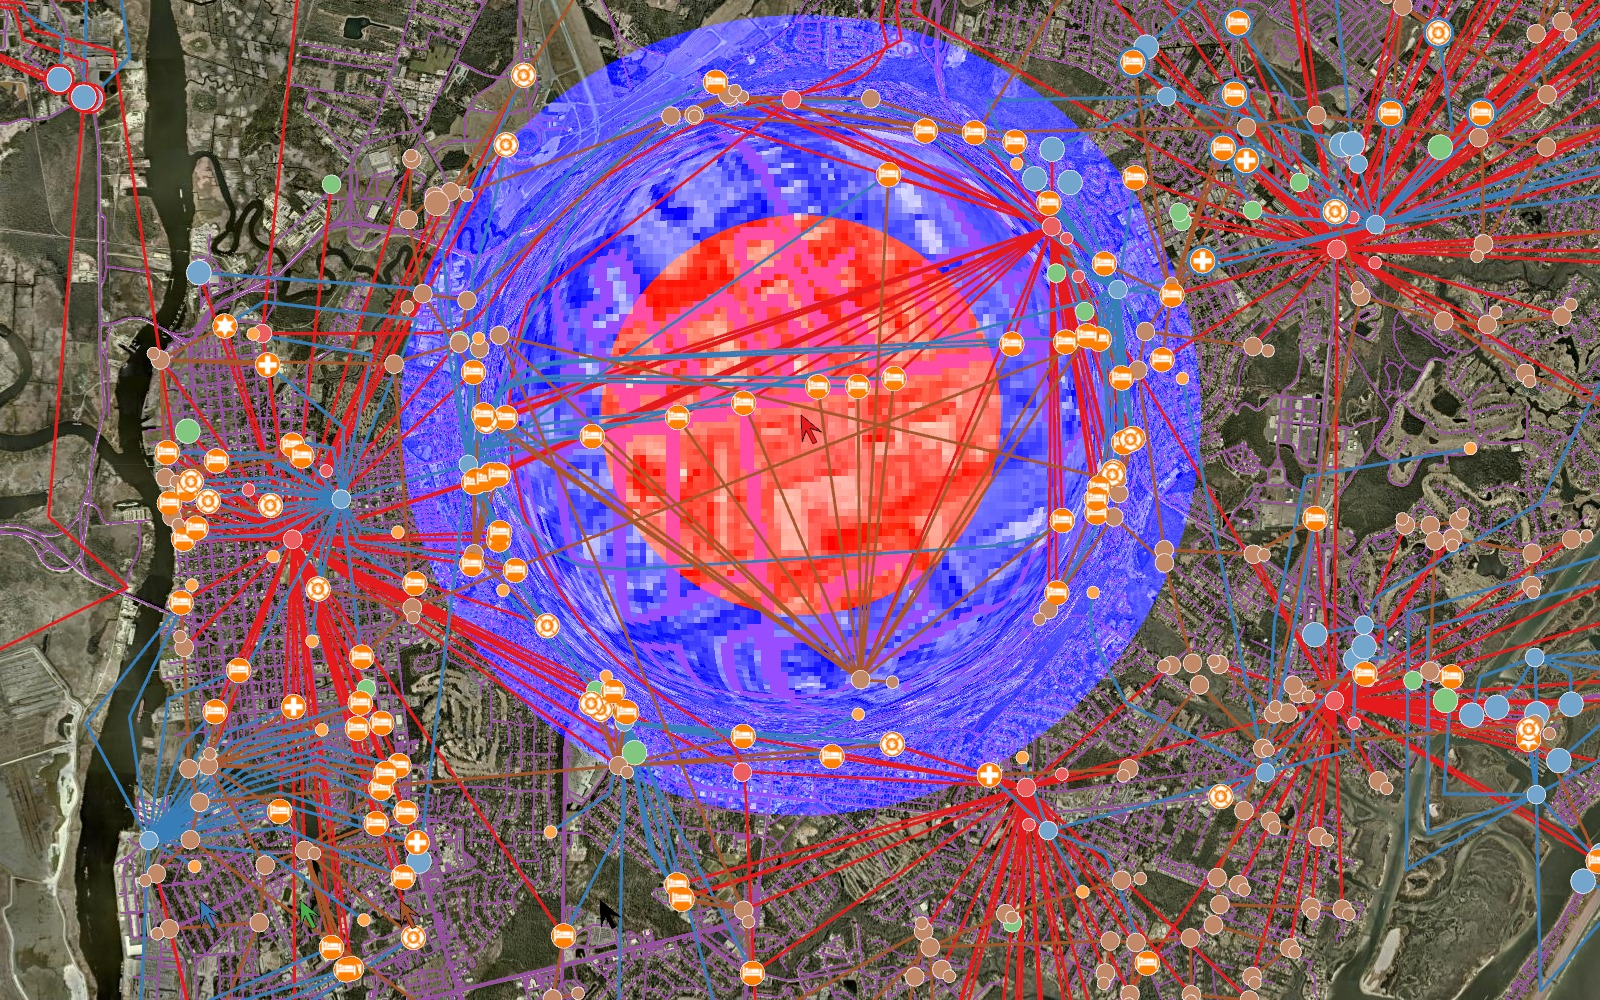
\includegraphics[width=0.40\linewidth]{img/20_half_linear_color.jpg}
    \vspace{3 mm}
    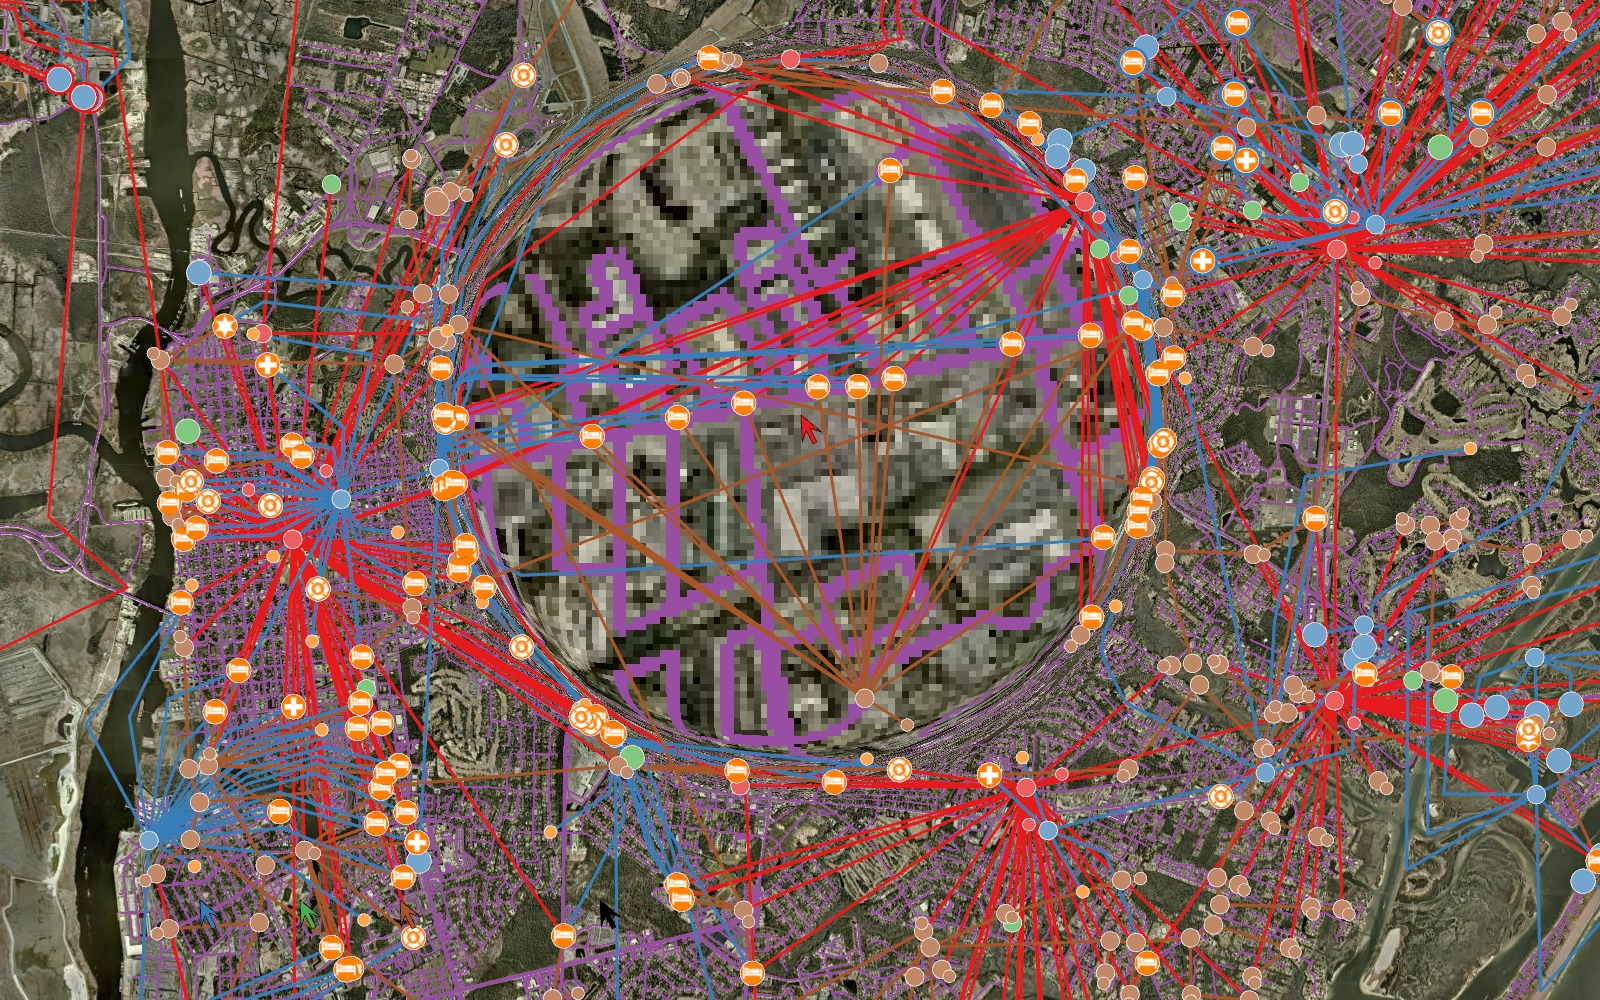
\includegraphics[width=0.40\linewidth]{img/20_three_quarter.jpg}
    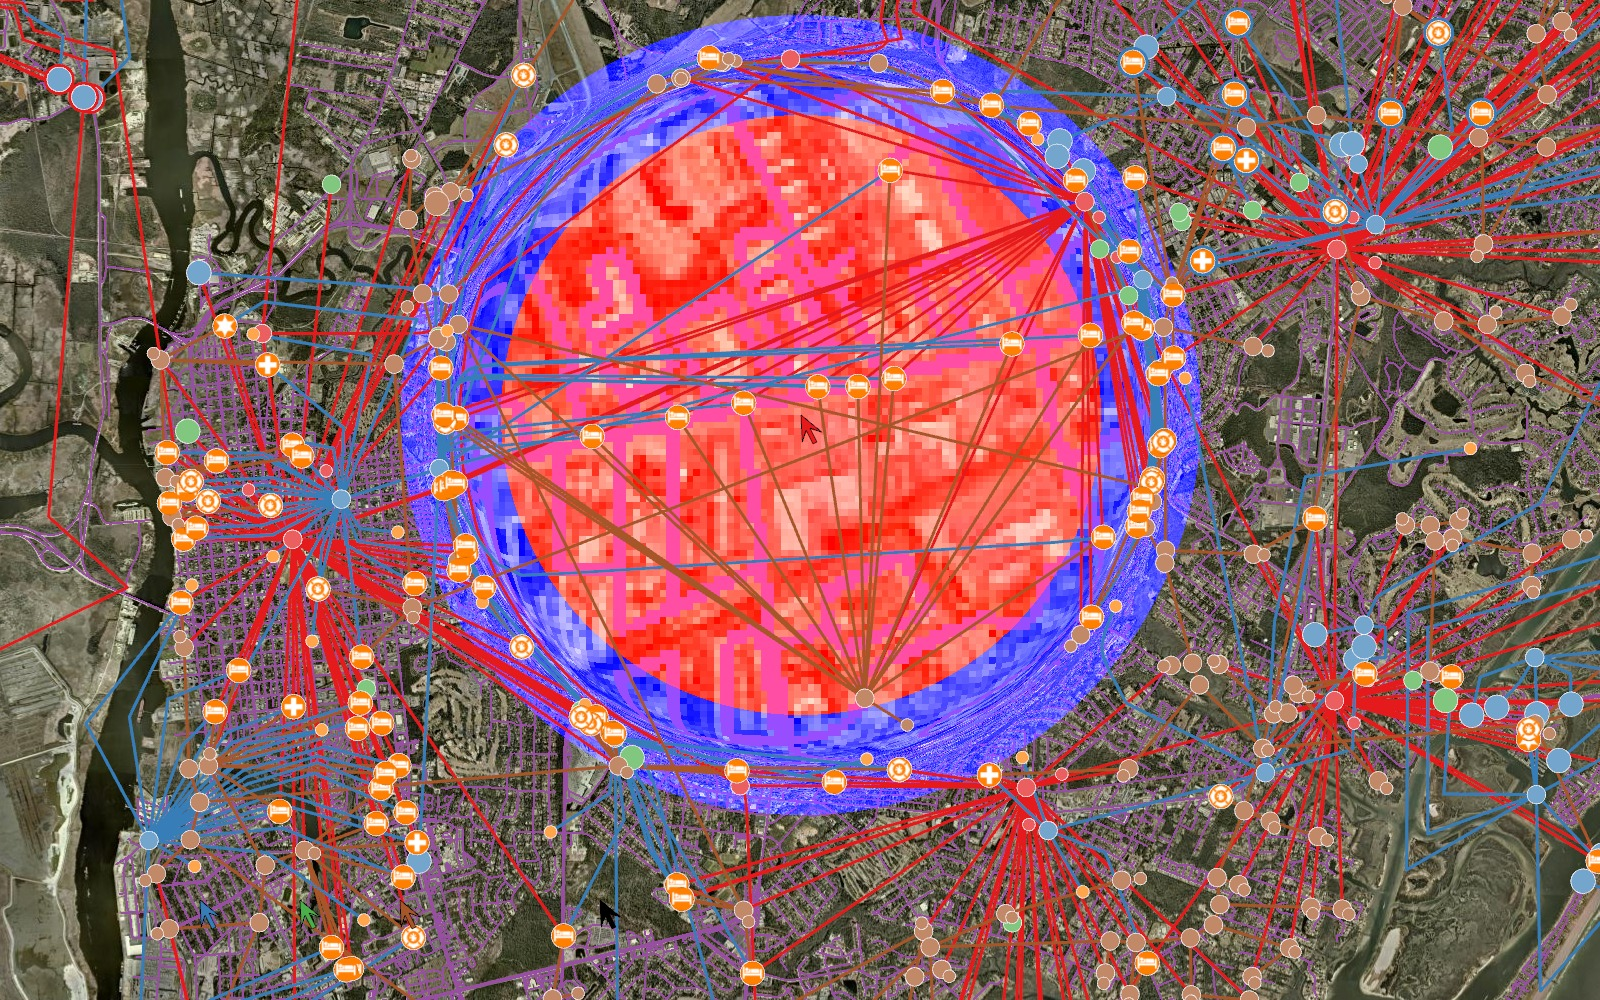
\includegraphics[width=0.40\linewidth]{img/20_three_quarter_color.jpg}
    \vspace{3 mm}
    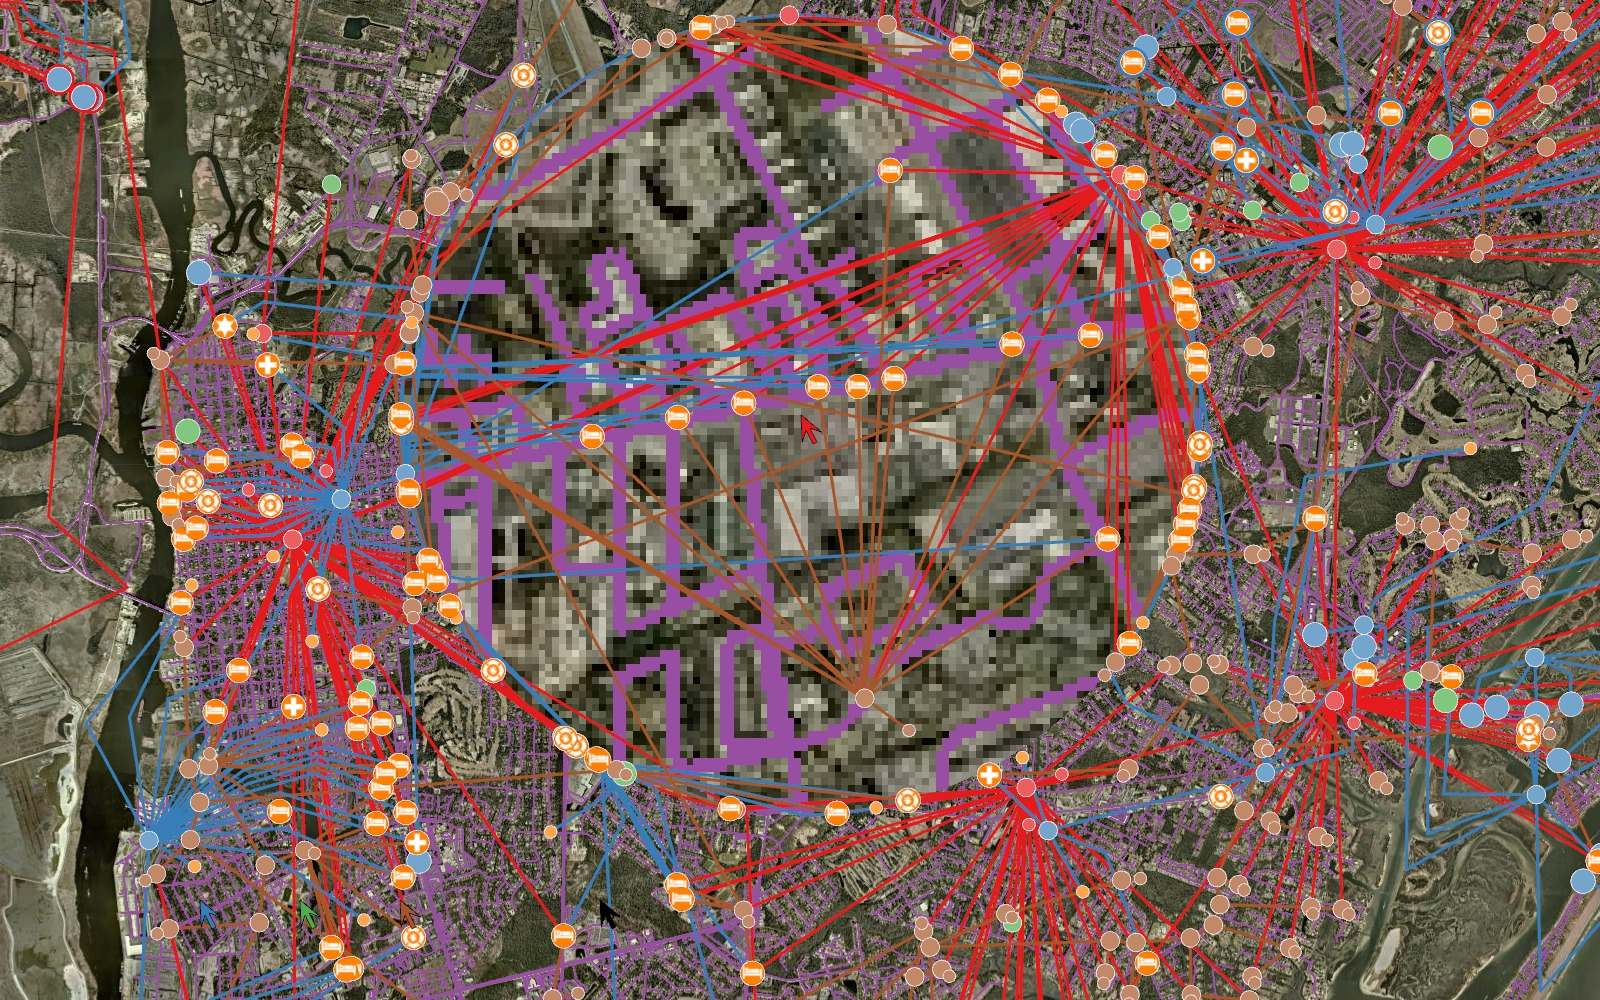
\includegraphics[width=0.40\linewidth]{img/20_only_linear.jpg}
    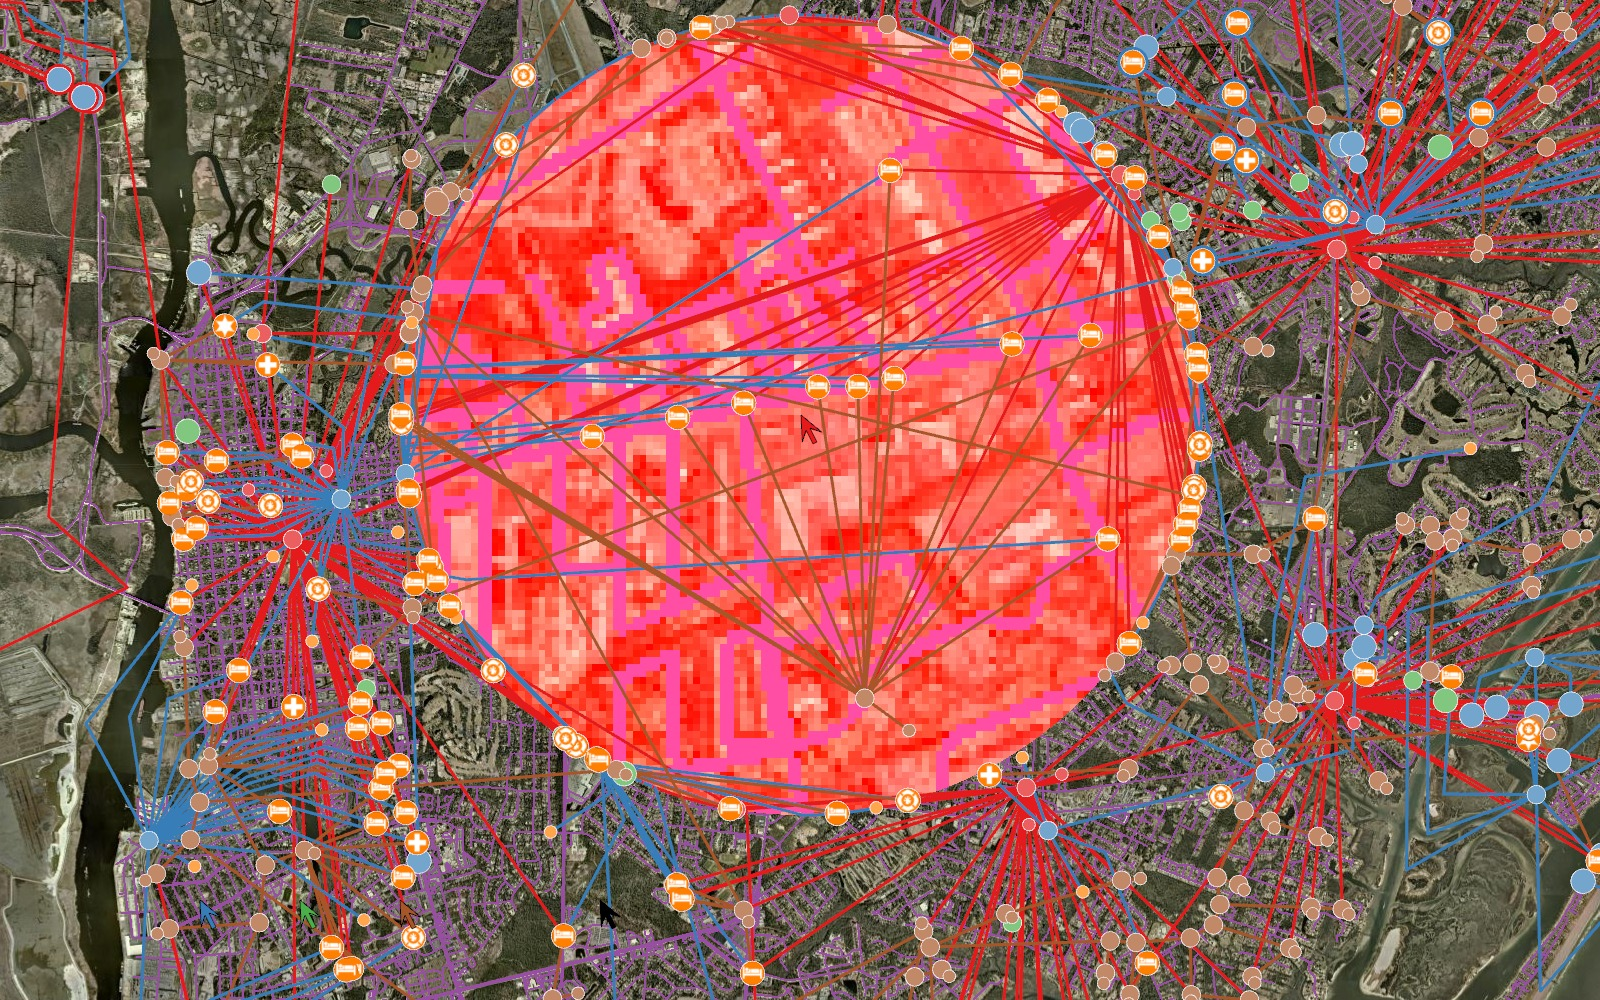
\includegraphics[width=0.40\linewidth]{img/20_only_linear_color.jpg}
    \caption[Various Inner and Outer Radius Ratios]{A series of images showing examples of different sized linear and non-linear magnification regions. As we increase the size of the linear region, the non-linear region becomes more and more distorted.}
    \label{fig:ratio}
\end{figure}
    

\section{Performance}
\label{section:performance_results}

Different aspects of the system were analyzed with regards to their performance. Each of the main individual systems: the satellite images, the road network, and the graph network were measured for the amount of time it took to complete a single render function of their respective data. 

For rendering the satellite images, we measured the amount of time it took to render to the FBO for a 1600 by 1000 resolution window\@. Figure~\ref{fig:satellite_graph} displays this information.  For the most part, rendering the satellite images takes less than 0.02 seconds no matter the number of tiles being rendered. Each tile is a 1024 by 1024 texture. The number of tiles on screen depends on the current level of detail of the overall application, as well as the positioning
within the application. The individual data points were simply measured by recording the amount of time a single render function call occurred, including the retrieval of the correct texture. The blue line in the graph shows the average amount of time it takes to render the satellite images with a specific number of tiles as the number of tiles increases.

\begin{figure}[htp]\centering
    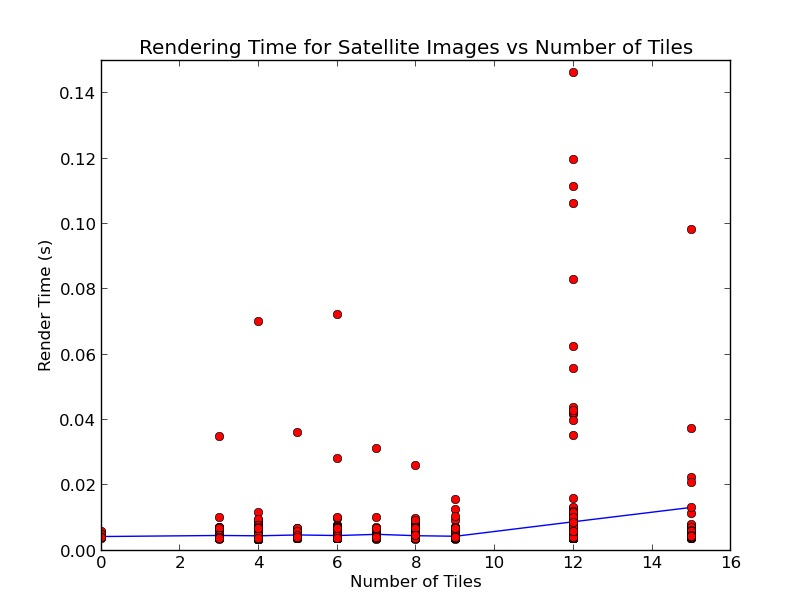
\includegraphics[width=0.80\linewidth]{img/satellite_render_graph.jpg}
    \caption[Satellite Image Render Time Graph]{The blue line represents the average amount of time it takes to render a given number of tiles. The red dots are individual data points. The outliers are likely due to the time the simulation takes to load a new image when viewing a different part of the map that is not already loaded into the cache.}
    \label{fig:satellite_graph}
\end{figure}

Table~\ref{table:road_and_graph_render_time} shows the average render time for the road network and graph network. Currently, neither the graph network nor the road network vary in size, so we simply calculate the average time for rendering for the current status of the system. Both take a relatively insignificant amount of time to render, even though the road network has roughly 640,000 vertices and the graph network has approximately 60,000 vertices being rendered.

\begin{table}[htp]
    \begin{center}
        \caption[Road and Graph Network Average Render Time]{The average time it takes to perform a render of the different elements for the current state of the system.}
        \label{table:road_and_graph_render_time}
        \begin{tabular}[H]{l | c | c}
                                & Number of Elements    & Time (ms)   \\
            \hline
            Satellite Images    & Up to 15              & 4.954 \\
            Road Network        & 33664                 & 0.492 \\
            Graph Network       & 2563                  & 6.409 \\
        \end{tabular}
    \end{center}
\end{table}

In addition to the graph network being measured in terms of render performance, we recorded the amount of time it took to perform the magnification functions on the graph network, nodes and edges are treated equally within this calculation, so the total number of elements is simply the sum of nodes and edges within the system. This is seen Figures~\ref{fig:one_mouse_data},~\ref{fig:two_mouse_data} and~\ref{fig:three_mouse_data}.

\begin{figure}[htp] \centering
    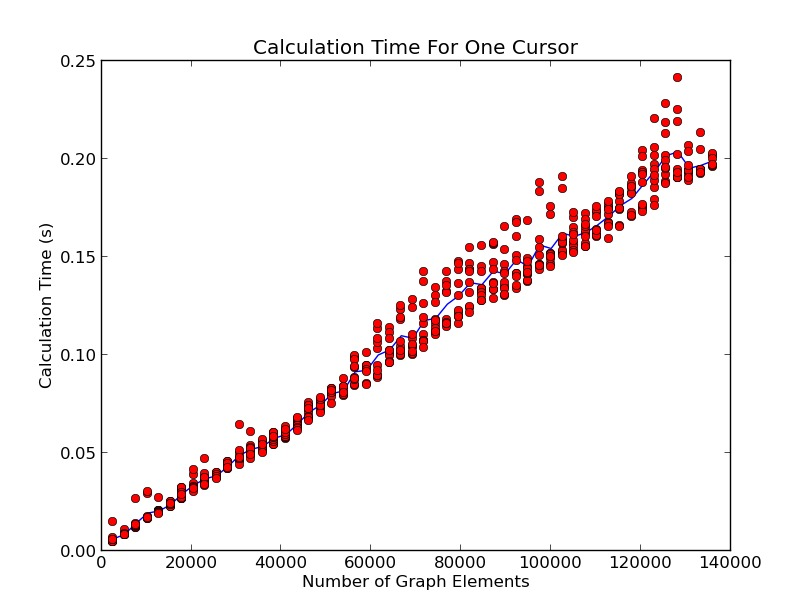
\includegraphics[width=0.60\linewidth]{img/one_mouse_move.jpg}
    \caption[Graph Magnification Calculation Time for One Cursor]{The red circles represent individual data points for a given amount of graph elements. The blue line simply shows the average, but there are relatively few outliers, and the graph clearly shows that the correlation between the number of elements and the time required to perform the movement function is roughly linear.}
    \label{fig:one_mouse_data}
\end{figure}
\begin{figure} \centering
    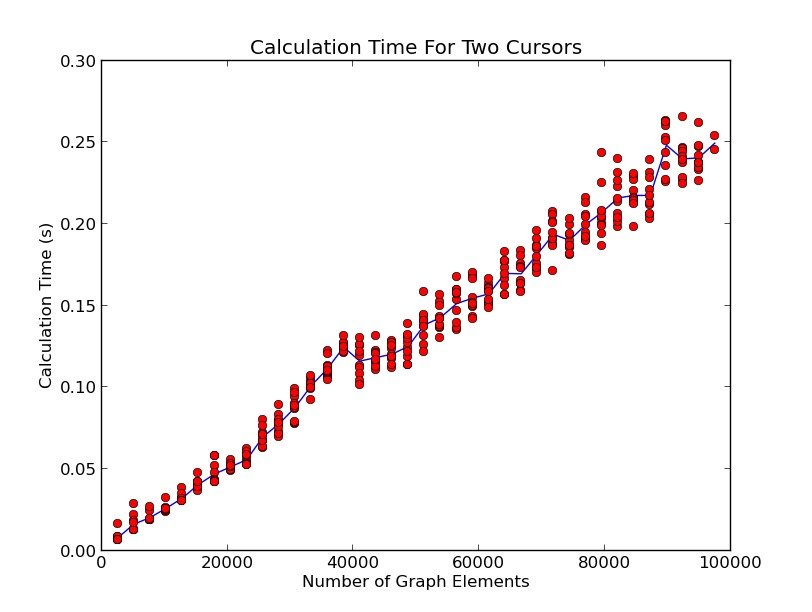
\includegraphics[width=0.60\linewidth]{img/two_mouse_move.jpg}
    \caption[Graph Magnification Calculation Time for Two Cursors]{Like the previous figure, the correlation is roughly linear between the number of elements and the time required. Adding an additional cursor increases the rate of growth of the function.}
    \label{fig:two_mouse_data}
\end{figure}
\begin{figure}[htp] \centering
    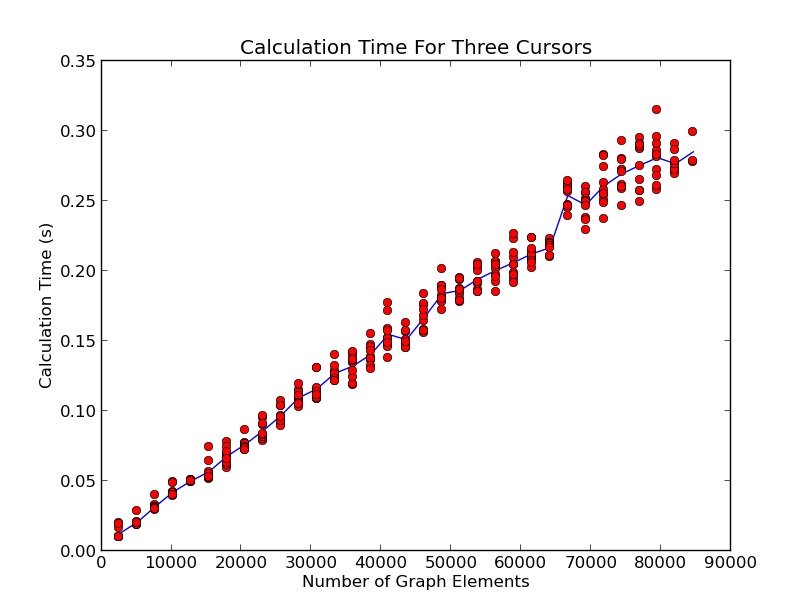
\includegraphics[width=0.60\linewidth]{img/three_mouse_move.jpg}
    \caption[Graph Magnification Calculation Time for Three Cursors]{An additional cursor keeps the linear correlation between the number of elements and calculation time. We also see that the extra cursor further increases the growth rate of the function.}
    \label{fig:three_mouse_data}
\end{figure}

Currently, the system runs with 808 nodes and 1755 edges for a total of 2563 elements. Even with roughly ten times as many data elements, it only takes 0.08 seconds for one, two, or three cursors. Increasing the number of cursors within the system causes a linear growth in the amount of time it takes to perform the magnification. It may be possible to make this growth sub-linear by utilizing the existing quad-tree data structure. This was simulated by duplicating the elements within the graph network, as we do not have a dataset that contains more than 2563 elements. It is unlikely
that we would need work with a data set much bigger than 200,000 elements. Assuming that elements are evenly distributed, we would have a region that covers 100 times the area - resulting in a simulation for a region that would be handled by more than a single team of emergency response officials.

The gDEBugger application was also used to measure global aspects of the visualization's performance \cite{gdebugger_website}. Memory usage of the application can be seen in Table~\ref{table:memory}. Figure~\ref{fig:fps_graph} shows a graph of the frames per second (FPS) for the application over the first thirty seconds of runtime.

\begin{figure}[htp] \centering
    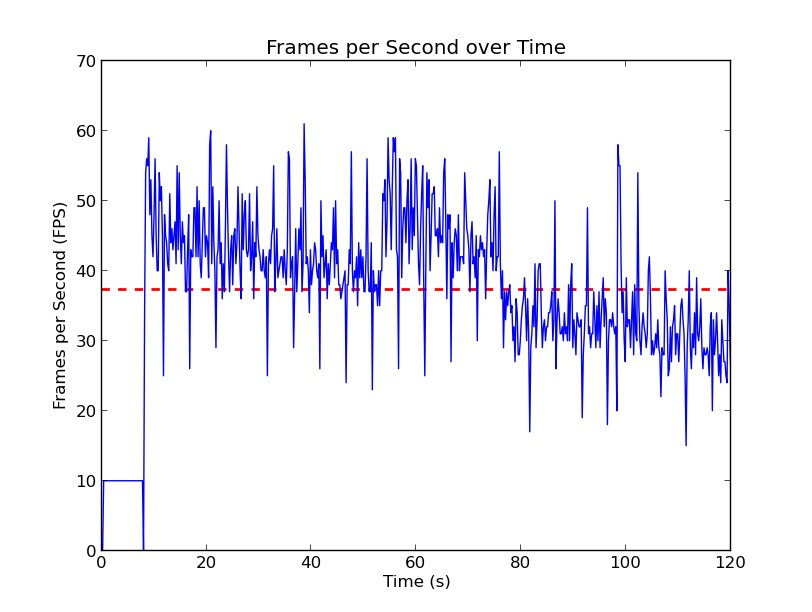
\includegraphics[width=0.80\linewidth]{img/FPS_graph.jpg}
    \caption[Overall Application FPS]{The red line shows that the average FPS over the first 20 seconds is 37.23 FPS\@. The initial low FPS is due to the application taking a few seconds to load data from the database which blocks all rendering.}
    \label{fig:fps_graph}
\end{figure}

The system maintains an interactive framerate, with only a few instances of the FPS dipping below 30. Even with these dips in framerate, this should not hinder the usage of the overall application, as users will probably not be continually interacting with the system.

\begin{table}[htp]
    \caption[Memory Usage]{The memory usage of the OpenGL relevant portions of the application is displayed. Textures take up approximately 50\% of the data being stored. Overall, the application uses a relatively small amount of GPU data, only 107 MB total.}
    \label{table:memory}
    \begin{center}
        \begin{tabular}[H]{l | r | c}
            Object Type     & Memory Size   & \# of Objects \\
            \hline
            Shaders         & 43 KB         & 32  \\
            Shading Programs& Insignificant & 13  \\
            VBOs            & 21956 KB      & 54  \\
            FBOs            & Insignificant & 1   \\
            Textures        & 49905 KB      & 17  \\
            Static Buffers  & 35941 KB      & 8   \\
            \hline
            Total           & 107845 KB     & 125 \\
        \end{tabular}
    \end{center}
\end{table}

The textures containing satellites are the biggest contributor of memory within the system, followed closely by the static buffers and the VBOs. We frequently update the texture and VBO data, so it may be prudent to try and reduce the amount of data being stored for VBOs. Because this application only takes up 107 MB of data on the GPU, it should run on pretty much any hardware. Dedicated GPUs usually have between 1 GB and 4 GB of memory, and integrated GPUs use the regular system RAM.

\section{Survey and Discussion}
\label{section:user_survey}

An informal survey of fellow students was performed for preliminary feedback on the changes proposed in Chapter~\ref{chapter:magnification} with regards to using the overall application. The different participants were given time to interact with the map for five minutes using the traditional methods of global zooming. After this time period passed, they used the new focus plus context system, and their opinions and thoughts about the two different methods of interaction were
recorded.

\begin{itemize}
    \item Magnification looks intuitive, seems like holding a magnifying glass.
    \item Magnification draws eyes to the magnified area.
    \item Cursor magnification instead of traditional zooming useful due to global information.

    \item Combined areas of magnification look weird, but unsure what should be displayed.

    \item With high magnification, mouse interaction is too sensitive.
    \item Some edges being magnified while others aren't is distracting.
    \item Difficult to click on elements due to how the nodes move around, try applying a different effect instead of just moving them.
\end{itemize}

The fact that the participants found the visualization helpful was expected due to the application requiring a global overview of the entire data to formulate solutions. The responses related to the actual interaction with the system were surprising. Due to my familiarity with the system, I did not notice that graph elements changing their screen position was initially a difficult concept to grasp, as the elements initially move away as you approach them. The oversensitivity of the interaction was expected, as it was difficult to control even when debugging.

In a formal study, it is  important to get quantitative data about user interaction with the system and the overall usefulness of the visualization. By logging the actions that a user takes while interacting with this system, an experiment could be designed to measure the number of actions a user needs to take to perform a task within the system. We could measure the amount of distance that the
mouse cursor travels and count the number of actions performed to quantify the usability of the entire visualization. Having lower values for both would indicate that the user was able to see more data and was assisted by the overall system. 

\section{Summary}
\label{section:results_summary}

This chapter presented a series of figures showing the magnification of the satellite images and graph network with single and multiple cursors interacting with the system. We also discussed various performance statistics related to rendering and performing magnification operations on the CPU\@. Finally, we detailed the results of a brief survey of inexperienced users regarding the visual effects of the system and their interaction. The following chapter will discuss possible future
work stemming from this thesis.

